\documentclass[12pt]{article}

\usepackage{hyperref}
\hypersetup{
	colorlinks,
	citecolor=blue,
	%filecolor=black,
	linkcolor=black,
	urlcolor=blue
}
\usepackage{float}
\usepackage[english]{babel}
\usepackage[square,numbers]{natbib}
\bibliographystyle{abbrvnat}
\usepackage{url}
\usepackage[utf8x]{inputenc}
\usepackage{amsmath}
\usepackage{graphicx}
\graphicspath{{images/}}
\usepackage{parskip}
\usepackage{fancyhdr}
\usepackage{vmargin}
\PassOptionsToPackage{hyphens}{url}\usepackage{hyperref}
\setmarginsrb{3 cm}{2.5 cm}{3 cm}{2.5 cm}{1 cm}{1.5 cm}{1 cm}{1.5 cm}
\usepackage[table]{xcolor}
\usepackage{todonotes}
\usepackage{menukeys}

\title{Android Application for leasing residences}   
% Title
\author{ Chrysoula Themeli, M1423\\
	Vassiliki Moschou, M1507}                               % Authors
\date{\today}                                           % Date

\makeatletter
\let\thetitle\@title
\let\theauthor\@author
\let\thedate\@date
\makeatother

\pagestyle{fancy}
\fancyhf{}
%\rhead{\theauthor}
\lhead{\thetitle}
\cfoot{\thepage}

\begin{document}
	
	\begin{titlepage}
		\centering
		\vspace*{0.5 cm}
		
\includegraphics[scale = 0.75]{ekpalogo.png}\\[1.0 cm]   % University Logo
		\textsc{\LARGE National and Kapodistrian University of Athens}\\[2.0 cm]   % University Name
		\textsc{\Large Department of Informatics and Telecommunications}\\[0.5 cm]               % Department
		\textsc{\large E-Commerce Technologies}\\[0.5 cm]               % Course Name
		\rule{\linewidth}{0.2 mm} \\[0.4 cm]
		{ \huge \bfseries \thetitle}\\
		\rule{\linewidth}{0.2 mm} \\[1.5 cm]
		
		\begin{minipage}{0.4\textwidth}
			\begin{center} \large
				\theauthor
			\end{center}
		\end{minipage}~
		\begin{minipage}{0.4\textwidth}
		\end{minipage}\\[2 cm]
		
		{\large \thedate}\\[2 cm]
		
		\vfill
		
	\end{titlepage}
	
	%%%%%%%%%%%%%%%%%%%%%%%%%%%%%%%%%%%%%%%%%%%%%%%%%%%%%%%%%%%%%%%%%%%%%%%%%%%%%%%%%%%%%%%%%
	
	\tableofcontents
	\listoffigures
	\newpage
	
	%%%%%%%%%%%%%%%%%%%%%%%%%%%%%%%%%%%%%%%%%%%%%%%%%%%%%%%%%%%%%%%%%%%%%%%%%%%%%%%%%%%%%%%%%
	
	\section{Introduction}
	
	In order to meet the requirements of the course of E-commerce Technologies, an Android application for booking rooms/residences was implemented, following the logic of the known Airbnb application. This report includes a short definition and description of E-commerce characteristics, as well as the purpose of developing this application. There is a thorough analysis of any important decisions regarding the design process, the assumptions and all necessary details related to the project. 
	
	\subsection{Description of E-commerce}
	
	%introduction, description of e-commerce
	
	Electronic commerce (e-commerce) is a type of a business model, or a segment of a larger business model, that enables a firm or an individual to conduct business over an electronic network, typically the Internet. Electronic commerce operates in all four of the major market segments: business to business, business to consumer, consumer to consumer and consumer to business. Almost any product or service can be offered via e-commerce, from books and music to financial services and plane tickets. E-commerce has allowed firms to establish a market presence, or to enhance an existing market position, by providing a cheaper and more efficient distribution chain for their products or services.
	
	There are several types of electronic commerce. The most common is business to consumer, in which a business sells products or services directly to consumers over the Internet. An example of a business to consumer e-commerce transaction would be to individually purchasing a pair of sneakers through Nike's website. As of business to business type of electronic commerce, companies can sell their products or services to other companies over the Internet. An example would be the company GoDaddy, which sells domain names, websites, and hosting services to other businesses. Consumer to business electronic commerce involves consumers selling products or services to businesses. You've taken part in this form of e-commerce if you've ever completed an online payment survey where you've given your opinion about a product. Finally, regarding consumer to consumer e-commerce, consumers can sell products to other consumers via a website such as Amazon or eBay.
	
	The rise of e-commerce forces IT personnel to move beyond infrastructure design and maintenance and consider numerous customer-facing aspects such as consumer data privacy and security. When developing IT systems and applications to accommodate e-commerce activities, several things must be taken into consideration, like data governance related regulatory compliance mandates, personally identifiable information privacy rules and information protection protocols.
	
	Some benefits of e-commerce include its around-the-clock availability, the speed of access, the wide availability of goods and services for the consumer, easy accessibility, and international reach. Its perceived downsides include sometimes-limited customer service, consumers not being able to see or touch a product prior to purchase, and the necessitated wait time for product shipping.
	
	\subsection{Purpose of the application}
	
	As described above, e-commerce has changed the way commerce is performed for both products and services. One of the fields affected by e-commerce is tourism. Many sites and applications are implemented in order to facilitate all relevant services and transactions, like Booking, TripAdvisor, Airbnb, Trivago etc.
	
	The purpose of this project is the development of an Android Application for booking rooms/residences, enabling users to lease or rent short-term lodging including vacation rentals, apartment rentals, homestays, hostel beds, or hotel rooms. Therefore, in this application each user can have two roles. Once someone is registered, by default has the tenant (user) role. This means that he can search a residence, make a reservation, review/comment, check the inbox and send messages etc. However, there is also the ability to take over the role of host and upload information regarding residences for booking, followed by specific characteristics and availability periods. Below, the design of the database, the RESTful services and all screens of the application are described further.
	
	\section{Connection Details}
	
	\subsection{MySQL Database}
	
	For the successful initialization of the application, eight tables have been created: users, searches, residences, images, reservations, reviews, conversations and messages. 
	
	\begin{itemize}
		
		\item \textbf{Users:} The fields of this table describe all necessary information for all the users registered into the application, both tenants and hosts.The mandatory fields, in order for the user to be valid, are: first name, last name, username, password and email. However, there is extra information that can be filled out later by the user. The role of each user (tenant or host) doesn't need to be stored in the database, as it is a logic inherited from the functionality of the Android project, which will be analyzed further.
		\item \textbf{Searches:} This table was created in order to maintain all location searches that the user performs. This information is used at the Home Activity where application shows to user some recommendations of residences, based on search history.
		\item \textbf{Residences:} In this table all the residences, entered by hosts, are described. Specifically, the information stored is: the owner, the type (house, apartment, single room, etc), location details, short description and characteristics, cancellation policy, rules, available dates period and price information of the residence. The number of guests and rooms is used in order to calculate the availability for each day, since a residence may have more than one rooms and different tenants.
		\item \textbf{Images:} This table stores all the names of the images assigned and related to a specific residence. Therefore, the only necessary fields are: residence\_id and name. The location of these images is on the side of the server and will be analyzed further.
		\item \textbf{Reservations:} This table is used in order to store all data related to reservations that users have made. The main fields are: residence\_id, tenant\_id, host\_id, period and number of guests.
		\item \textbf{Reviews:} In the application, the user can rate and comment each visited residence. Therefore, a review table is needed to keep this information. The residence\_id and tenant\_id are obviously necessary here, as well as the comment and rating.
		\item \textbf{Conversations:} A message exchange pattern provides a direct communication between possible tenants or hosts, through their inbox. They can ask for details, instructions, give offers and have a formal conversation even before making a reservation. All messages are grouped based on the subject of the conversation, which is connected to the residence of the main interest. This restricts the users from sending messages irrelevant to the purpose of the application. Each user has access only to conversations that can be created through the environment of a residence, tenants can only send messages to the host, and the host can only start a conversation with the existing tenants. As a result, two tables are created. This is the first table, where the main fields are the sender's and receiver's (user) id, the subject of the conversation (which is basically the title of the residence assigned) and the id of the residence. Additionally, more information is provided, such as the creation date, and the conversation status set per user (read / deleted).
		\item\textbf{Messages:} In addition to the above, the second table is the messages table which stores the main content (body) and the timestamp of each message. This helps keeping in track every action of sending/receiving and make a proper ordering. Moreover, the messages are linked to a conversation ("conversations" table) based on the field "conversation\_id", in order for all the messages with the same subject to be grouped together. Similarly the deletion status per user is provided.
	\end{itemize}
	All above tables have a field id which is unique and auto-increment. 
	
	For our Database Model to become more clear, an Entity Relationship model was designed, showing only the most important fields of the Database, as per below:
	
	\begin{figure} [H]
		\begin{center}
			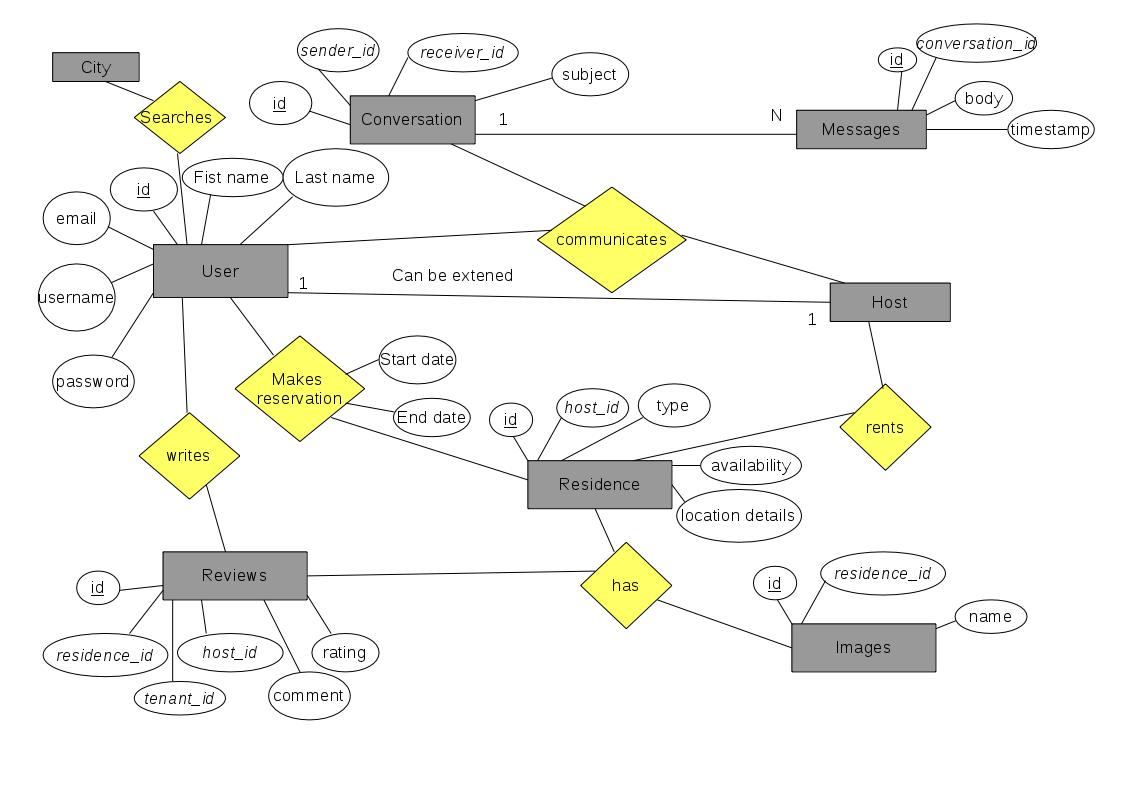
\includegraphics [scale = 0.55] {MonteloOntotitonSusxetiseon.jpg}
			\caption{Entity Relationship Model}
		\end{center}
	\end{figure}
	In above Model, all entities, their relationship and the main fields are shown. All primary keys are underlined and the foreign keys are emphasized with Italics. 
	
	Furthermore, the Enhanced Entity Relationship Model was extracted from MySQL Workbench, also showing the relations between the tables. 
	
	\begin{figure} [H]
		\begin{center}
			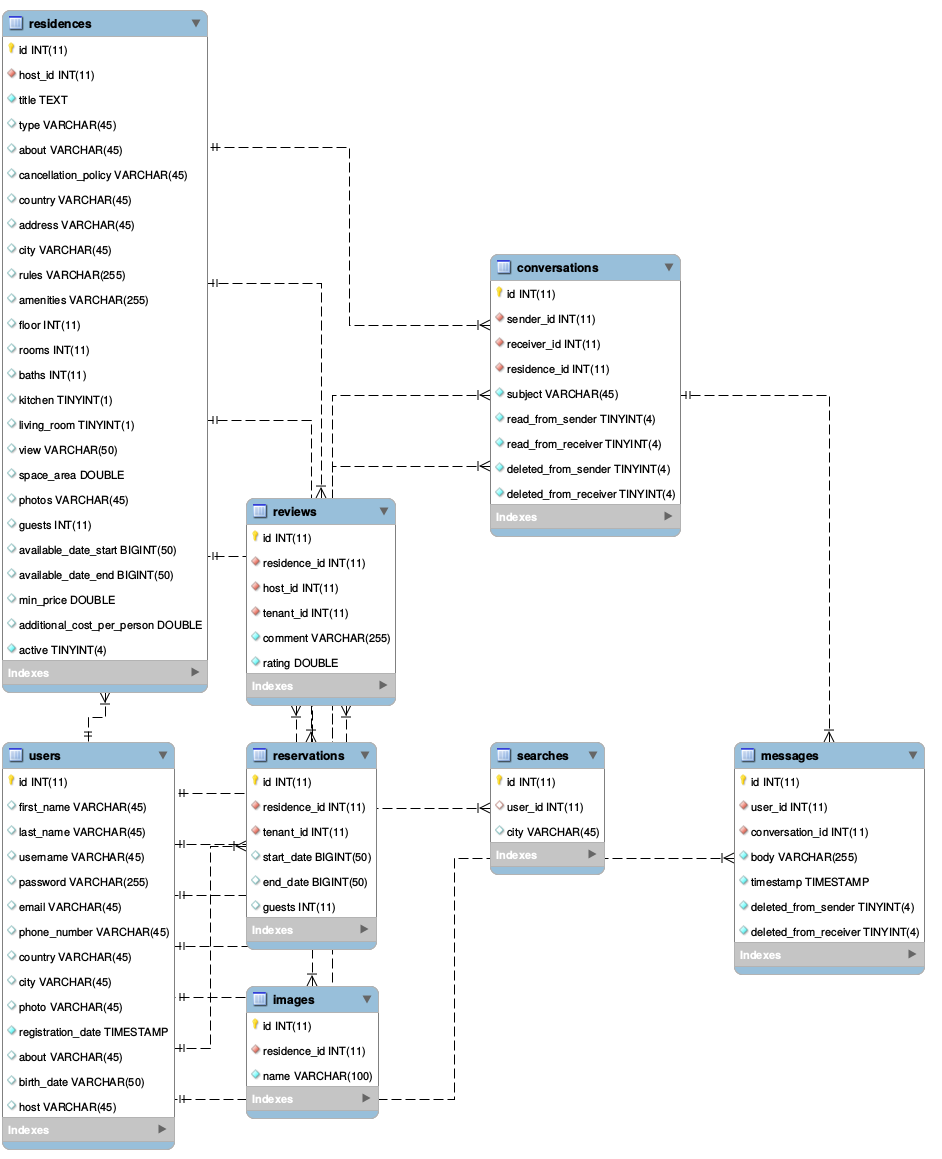
\includegraphics [scale = 0.40] {sxesiakomontelo.jpg}
			\caption{Enhanced Entity Relationship Model}
		\end{center}
	\end{figure}
	
	\subsection{RESTful Services}
	The way that the application communicates with the stored information, relies absolutely to the implementation of RESTful web services. REST describes any simple interface that transmits data over a standardized interface (such as HTTP). It provides an architectural set of design rules for creating stateless services that are viewed as resources, or sources of specific information (data and functionality). Each resource can be identified by its unique Uniform Resource Identifiers (URIs). Consequently, a client (either a consumer or a business) accesses a resource using only a URI that returns the proper information needed, in a specific format that the client can handle as they want. No extra keys or credentials are required for this connection as the permissions for this access have already been set between the client and the provider of the REST service.
	
	In the world of E-commerce there is a variety of such services (like REST, SOAP or XML-RPC) that serve easily and quickly all kind of needs that clients have. For example, an e-shop can integrate several types of services into its website or application, depending always on the documentation and the standards that each service provides.
	
	Analyzing the process of an online payment, when the buyer has selected their products and proceeds to checkout, they have to fill in the credentials of their credit card in order to be confirmed as valid users. If the validation is successful, the user makes the transaction and therefore completes the checkout procedure of the product. For this operation to be handled correctly, a connection with a payment web service has already been executed (for example a physical Bank or an online Payment Service - where the latter is supported to web services too). The website doesn't have any access to the payment account credentials of each user, that's why it must connect with a Web Service, enabling the users to withdraw their money from there, and continue their shopping into the website. 
	
	This procedure can be achieved with different ways, either by internal calls to the URIs of the web service through the website, or by redirection to the URIs of the Web Services that in this case, their return format, is a more user friendly environment that can guide the user to any completion steps presented. In this way, the domain of security is also supported, as each side (client and provider) has its own permissions specified, accessing only the data that is considered qualified. Even the techniques used by the clients for each Web Service can vary on the permissions restrictions and the level of the risk of vulnerability from attackers.
	
	Other cases that the Web Services work on, are the known electronic malls (e-malls) that use a variety of connections of plenty e-shops and collect information of all kinds of products grouped by price, brand etc. A real case is the \textit{Skroutz} web platform which provides URIs to its' clients in order for them to send their products list externally (in an XML format for example) and manage to be visible from other sources as well.
	
	\textbf{Connection with MySQL:} For the successful operation of the RESTful Web Service, specific methods that read or write on a database must be constructed, and share their result publicly. In more details, all the tables of the database are imported and used through MySQL queries. The desired return format that is used is JSON (could be XML, plain text, entity objects etc). In practice, for viewing the list of available residences provided into the Android application, a call to the Web Service is being made, asking for the list of all the residences (that have already been added through a similar way). Next, RESTful gets triggered, and makes a connection with the database through the domain entities representing the tables. It selects all the data from the table "residences", respecting any declared parameters or attributes, and the result (returned Array/Object/String etc) is converted to a serialized JSON value. Then it's up to the Android program to read this response, and handle it correctly. Below is shown a response of a REST call that brings all the available residences from the database.
	
	\begin{figure} [H]
		\begin{center}
			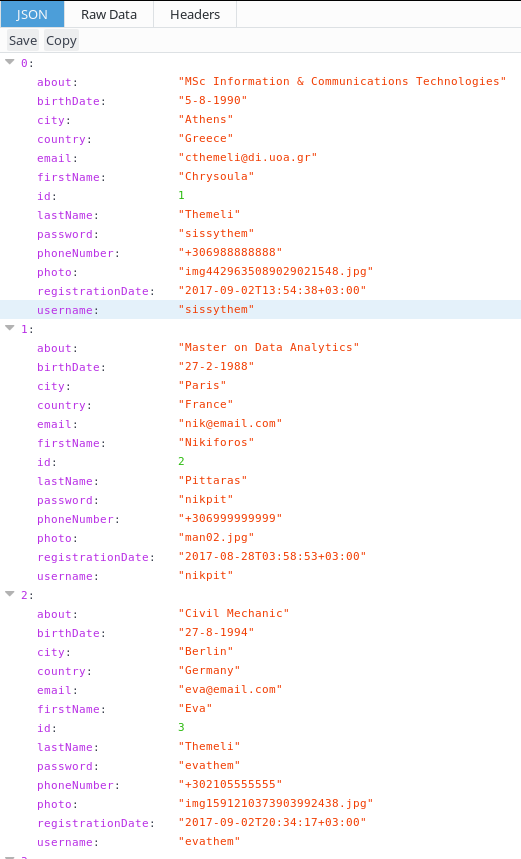
\includegraphics [scale = 0.35] {json.png}\\[1.0 cm]
			\caption{Sample of JSON response}
		\end{center}
	\end{figure}
	
	
	Something important that has to be mentioned, is the fact that the RESTful Web Service and the database should exist under the same technical environment / server, or at least under the same network. In this way, we can ensure the safety of the database, without having it open to the rest of the world and increase its vulnerability. The external client can be connected from everywhere, as it only needs a URI and the correct guidelines to make its application run (for the android application in this case, the apk file installed on their device).
	
	Finally, another requirement to be mentioned here, is that a session had to be created for each user and inform him when session is expired. For this purpose, in the Restful services side, two java classes are implemented: AuthenticationFilter and KeyHolder. In the first class, the method validateToken receives a variable token and checks if it is a signed and valid token. In the second class, the method issueToken creates a new token (this method is called in UsersFACADE for the calls related to login or register) and the method checkToken calls the method filter from the AuthenticationFilter class. This method finally calls the validateToken method to check the provided token. In all our calls, it is necessary that the application provides the token as header.
	
	\section{Android Application}
	
	In this section, all screens of the application will be described, including the design decisions and the functionalities used. 
	
	A crucial part of the project, is how our Android Application consumes these RESTful Services. Retrofit library is used for this purpose from the side of the Android application. Firstly, a class named RestClient is created, where the base external url of the RESTful Web Service is also declared. Through OkHttp it manages to communicate with the server using SSL. Moreover, RestAPI Interface has all the calls needed for the application together with the relevant anotations (@GET, @POST, @PUT, @DELETE) being set. Finally, the class RetrofitCalls has all the AsyncTasks and the accordant methods called from the activities. For POST/PUT requests, the necessary methods are implemented within the activity (methods separated from onCreate). 
	
	Several entity classes also present the data from database as Plain Java Objects (Users, Searches, Residences, Images, Conversations, Messages, Reservations and Reviews) giving the ability to compose the fields which will be passed through the calls. In order to handle these calls more efficiently, all JPA classes (RESTful side) have been implemented and adapted to the side of the Android project too. The result from GET is retrieved as an object of these classes. This decision has been made in order to avoid complicated containers to store all necessary information which made the code hard to understand.
	
	However, in ResidenceActivity it was necessary to make a REST call related to the map, in order to receive the latitude and longitude of the address and show it to the map. For this functionality, two classes have been created, the first one is called RestCallParameters class, which contains all the necessary information of a request, such as the URL, the request type (here is GET), the return type (JSON or Plain Text). In addition, a class named RestCallManager is implemented. This is a different thread from main, which runs in the background (method doInBackground), and once finished, returns the JSON Object or the text from the RESTful Services. When this thread runs, another method is called (getSingleJSONArray) which returns the result of the call.
	
	In order for the application to run correctly, there have been created some general classes which are used during the whole functionality and set some common properties for every method or activity in the project. The \textit{Session.java} Class represents a common Java Object which is triggered on every activity, in order to provide some common values stored via the Android SharedPreferences object. Through this object we can ensure that the preference values remain in a consistent state and control when they are committed to storage. More specifically, Session class stores the values of the \textit{username} of the user that has logged in to the application, the \textit{token} created from the RESTful Service indicating the validation of the user access (upon its' expiration) and the \textit{login status}, a boolean variable which remains true until the token expires. There is also the Utils.java class which is considered as a useful tool to implement methods that will be called from more than one activities and initialize the appropriate parameters, variables and constants only once. As a result, this class behaves as the activity itself thanks to the context parameters being passed on the call. Every important method and its' connection to related Activity will be analyzed further when needed. 
	
	After a successful first connection to the application, the user themselves have to handle all necessary permissions that are requested for approval (Internet access, location, images etc). Related to these permissions, we had to take into consideration the Android version of each device. More specifically, Android versions before 6 asked for permissions before downloding the application from Google Play, while the latest versions require permission's approval when the user enters for the first time in the application. Based on the permissions included in the Android Manifest, we added them into a Collection so as to check if permission is granted from user.
	
	\subsection{Register/Log in}
	
	\subsubsection{Greeting Activity}
	The first screen of our application is related to HomeActivity.java (activity\_home.xml is the relevant xml file). In this activity, it is checked whether the user is already logged in. In this case, they are welcomed to the main content of the home screen, otherwise they are redirected to the GreetingActivity.java (xml file: activity\_greeting.xml), which welcomes the user to the application and gives them the choice either to log in, if they have already an account, or to register. This is handled in combination with the SharedPreferences, as mentioned above. When a user logs in or registers successfully, the relevant username and the token (the response returned from REST) are stored to the SharedPreferences and passed from Home to every other activity through navigation. In addition, this information is added in onResume and onRestart android methods, therefore the user stays always logged in from the beginning of the application, until the expiration of the token (checked from REST), where they need to login again.
	
	From GreetingActivity, the user can only have access either to Register or Login activities. If they press the back button of their device, they can minimize the application, but they can never go to HomeActivity without previously having logged in or registered. The same logic is followed in HomeActivity and HostActivity screens. The first activity is the home page presented when the user has the role of tenant, while the second is for the host role. In both of these activities when the user goes back, the application is minimized.
	
	% Greeting Activity screenshot 
	\begin{figure} [H]
		\begin{center}
			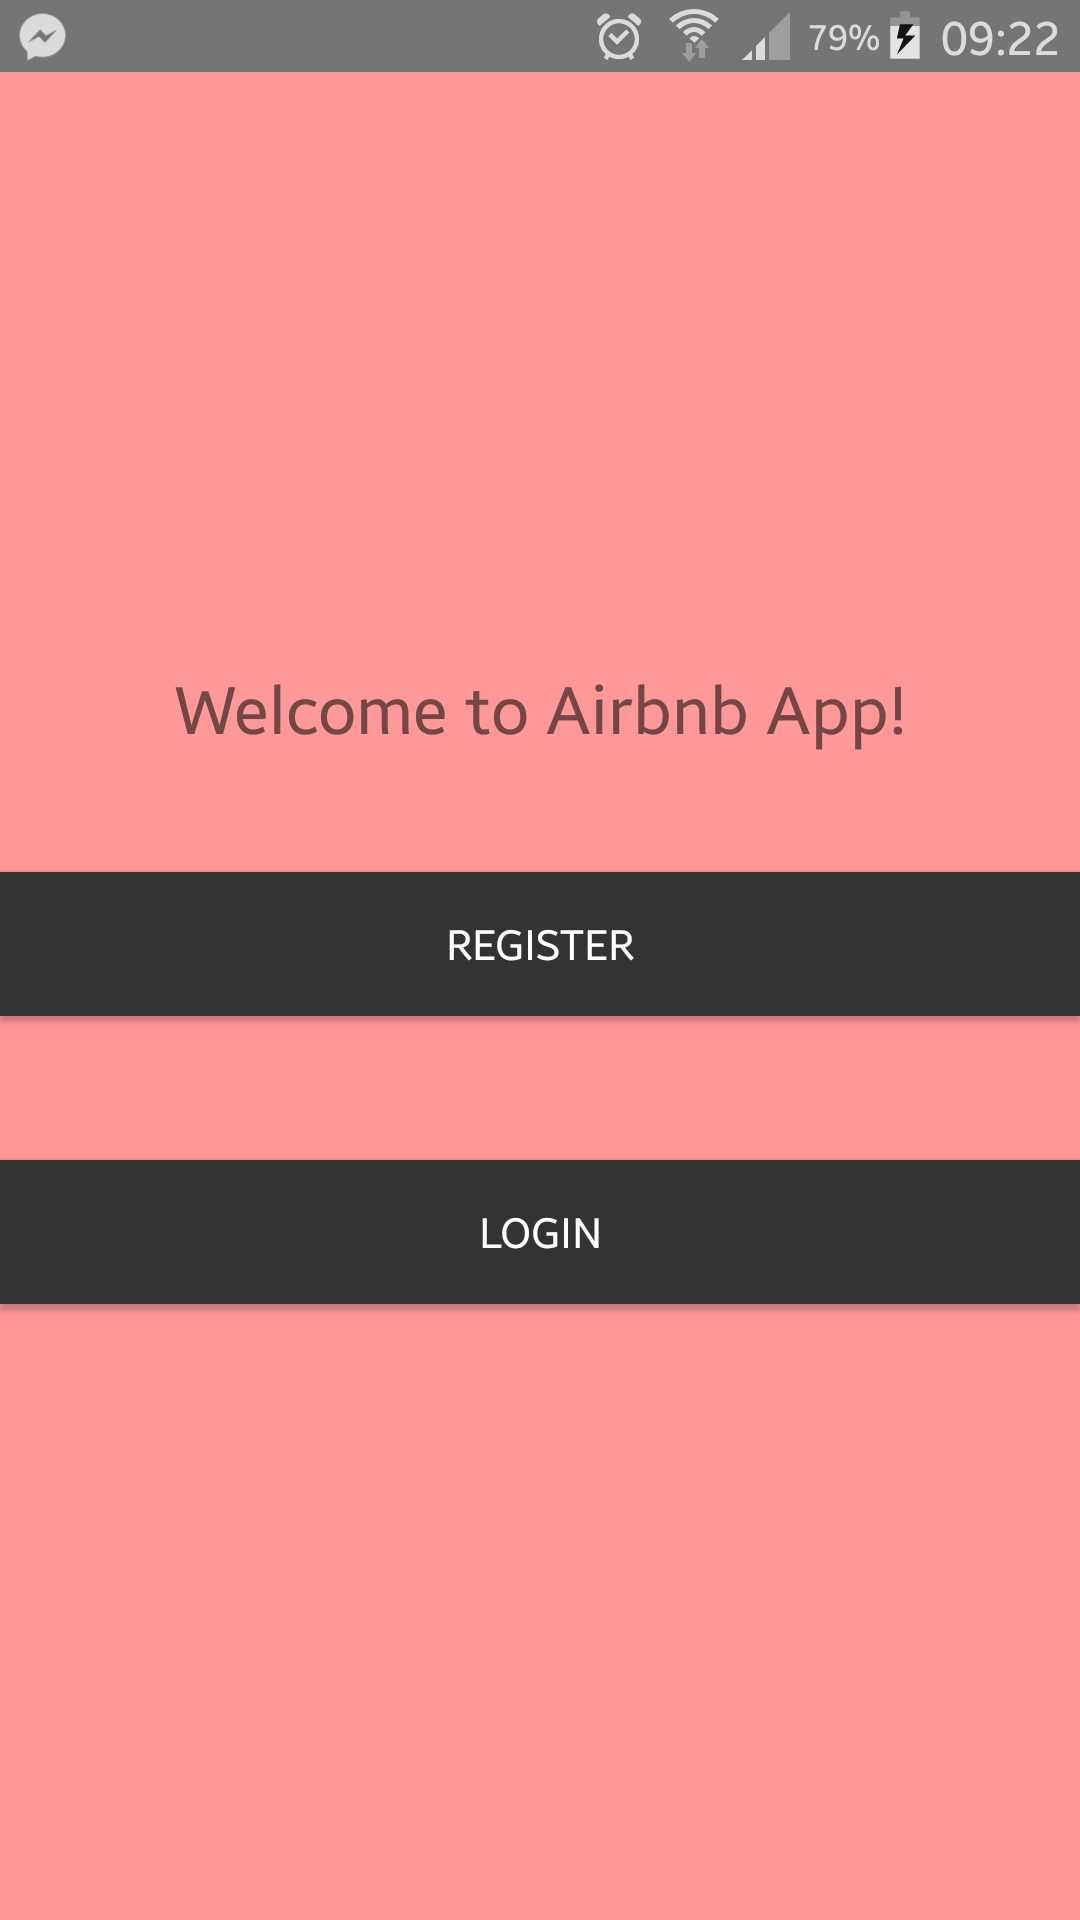
\includegraphics [scale = 0.13] {01-greetingActivity.png}\\[1.0 cm]
			\caption{Greeting Activity}
		\end{center}
	\end{figure}
	
	The data passed to HomeActivity are: username, login status and token. The Session Class is used here in order to hold all this information and pass it to all the activities as user navigates. In case of the expiration of the token, a logout method is called in order to clear the SharedPreferences and redirect the user to the GreetingActivity. As the HomeActivity is the first activity every user sees when they enter the app, the permissions functionality has been implemented in there and is called every time home is triggered. Of course, if the user has given permission to the actions needed, no notification message will appear to them again.
	
	\subsubsection{Register}
	When the user clicks on the Register button at the GreetingActivity, a new screen appears (RegisterActivity.java and activity\_register.xml) with mandatory fields to be completed by them. The fields are: first name, last name, email, username, password, confirm password and birth date. Our application, checks if all the fields are completed and also whether the password and confirmation password are identical. Our application checks if username and email are unique. In case one of these fields are found in the database, application does not let the user proceed and asks them to refill correctly either email or username field. 
	
	Finally, once the form is completed correctly, the user presses register button, and a POST request is sent to the database, in order to store the data to the respective table (users table). In order to send the POST request, android creates a JSON Object and provides it to the RESTful services. In this request, an object of the java entity is passed with all the fields of the user set, in order to be assigned to the entity of the RESTful Service. After a successful insertion into the database the token is created from the username of the new user. This is the main response that is returned and can be passed immediately to HomeActivity. Therefore, if the request was successful, the user proceeds to the Home screen.
	
	\subsubsection{Login}
	On the other hand, when user clicks the Login button, a corresponding form appears and asks them to fill in the username and the password (LoginActivity.java and activity\_login). Following a similar logic to the above process, a GET request is sent in order to check if username and password are correct. For this purpose, a MySQL query call is used via the @GET method in RESTful Service. If the credentials are wrong (based on the comparison between user input and response from server) an error message appears and fields should be filled again, otherwise the user is automatically logged in redirected to the Home screen. The main response of the login request is a String, indicating the token created. Therefore it is passed to SharedPreferences and the Session Class, and represents the key to all the next activities that will be called. If the user is invalid or the token is expired, the response will be \textit{null} or a String with either a value \textit{"not"} or \textit{""}.
	
	% Register & Login Activity screenshot 
	
	\begin{center}
		\begin{figure}
			\begin{tabular}{c c c}
				
				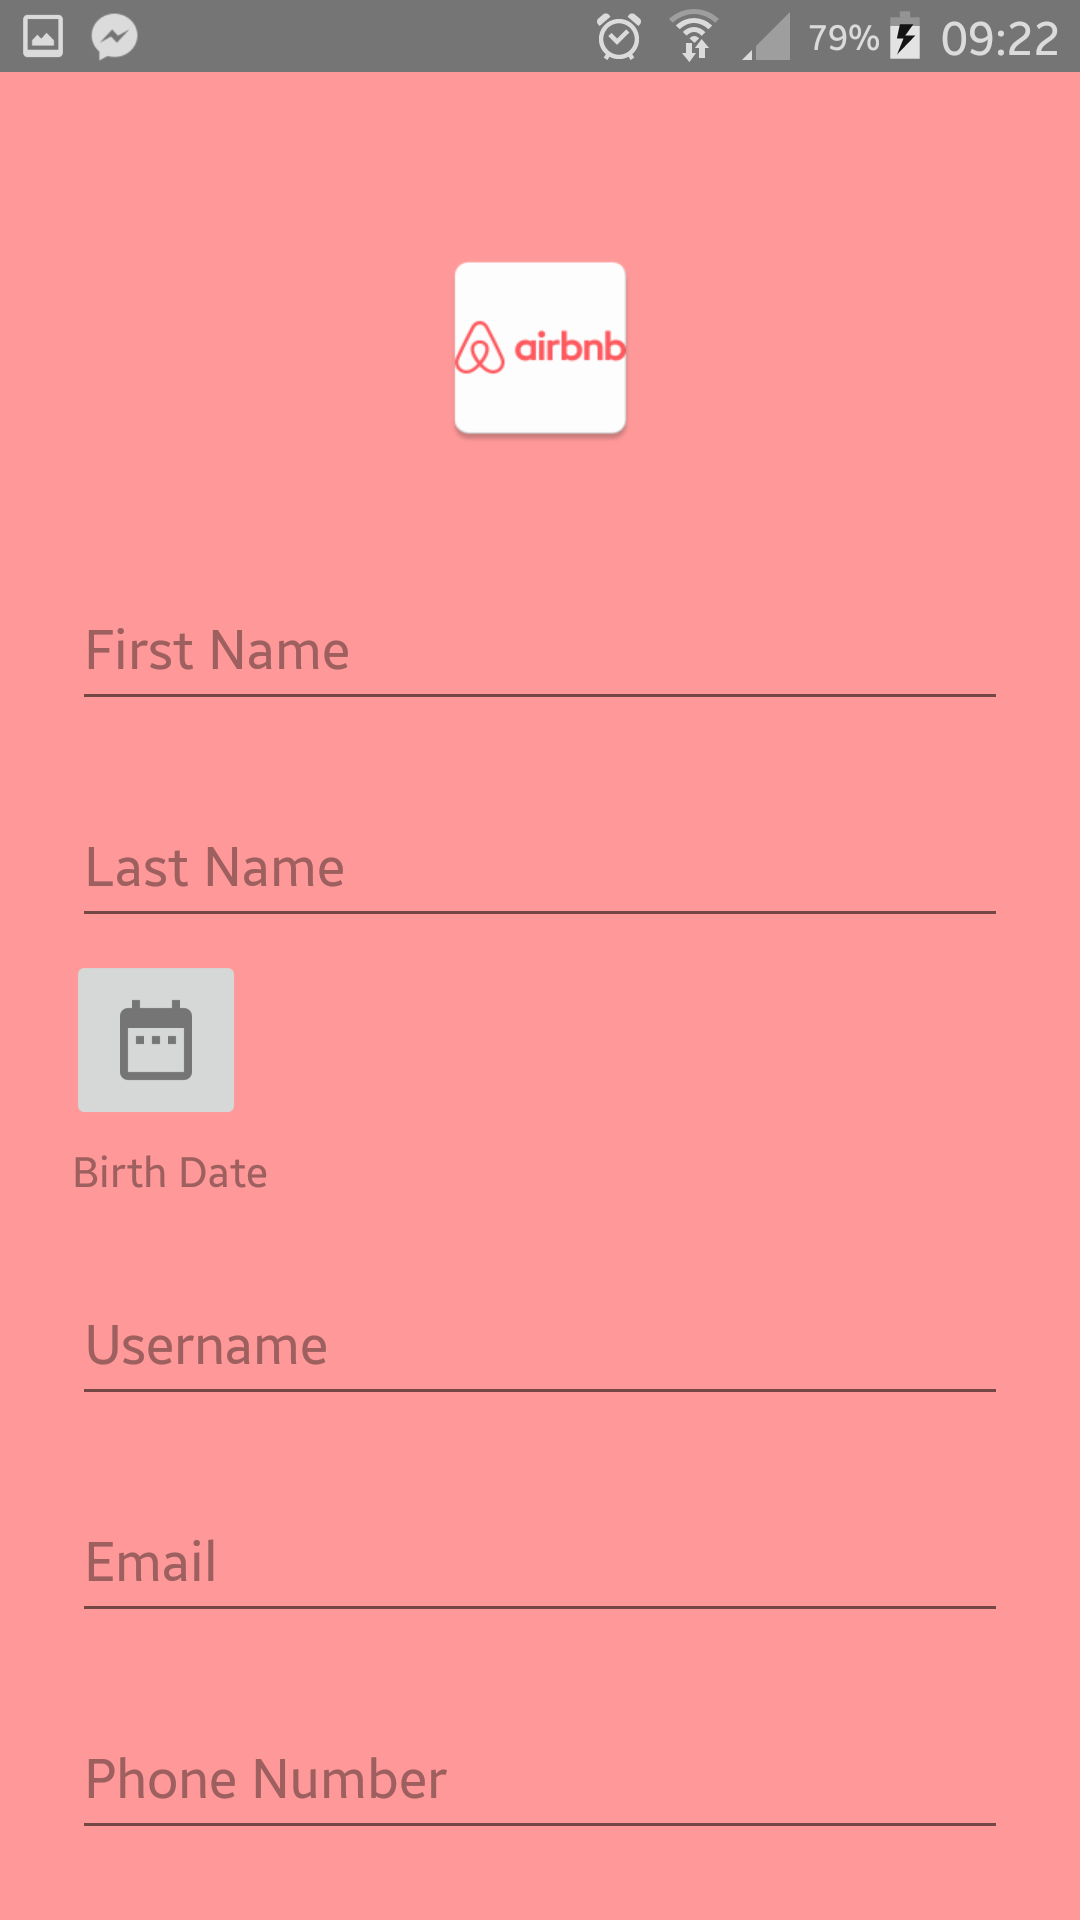
\includegraphics[scale=0.12, keepaspectratio]{02-register01.png}  
				&
				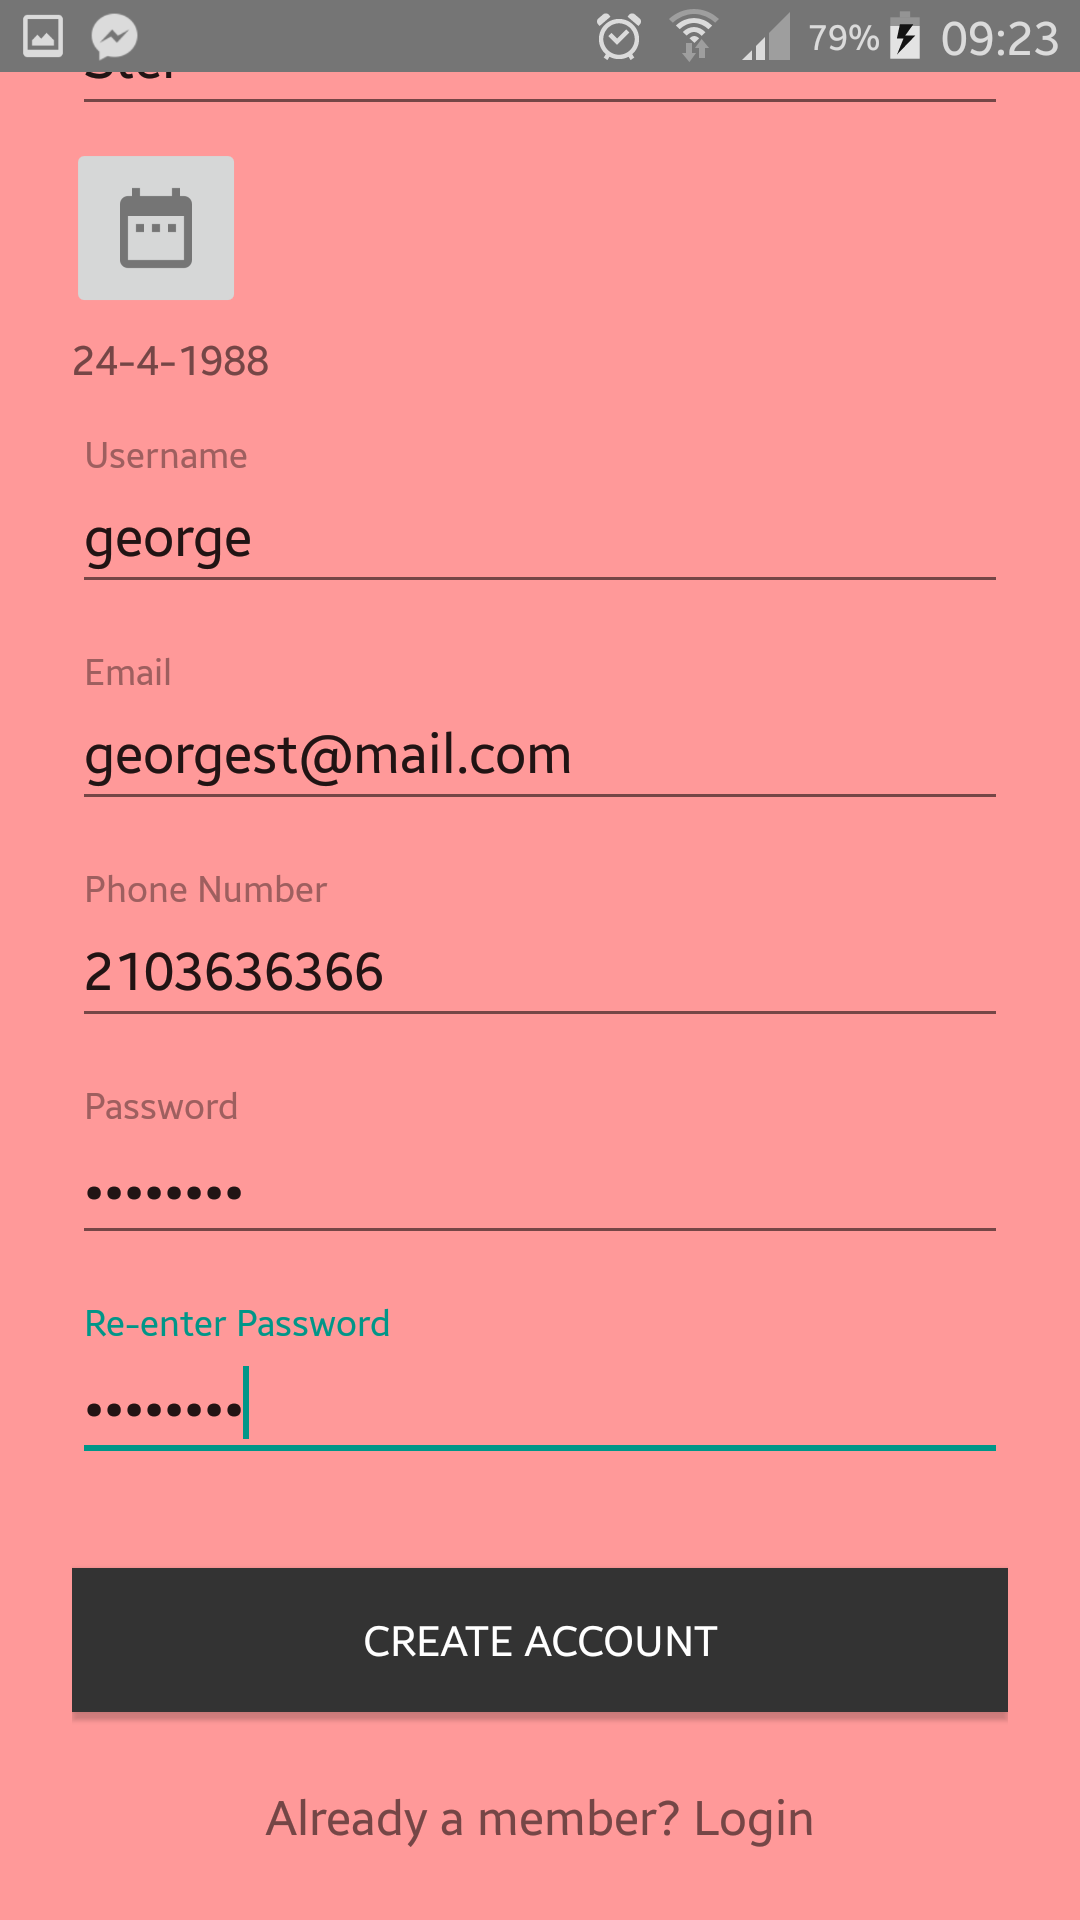
\includegraphics[scale=0.12, keepaspectratio]{03-register02.png}  
				&
				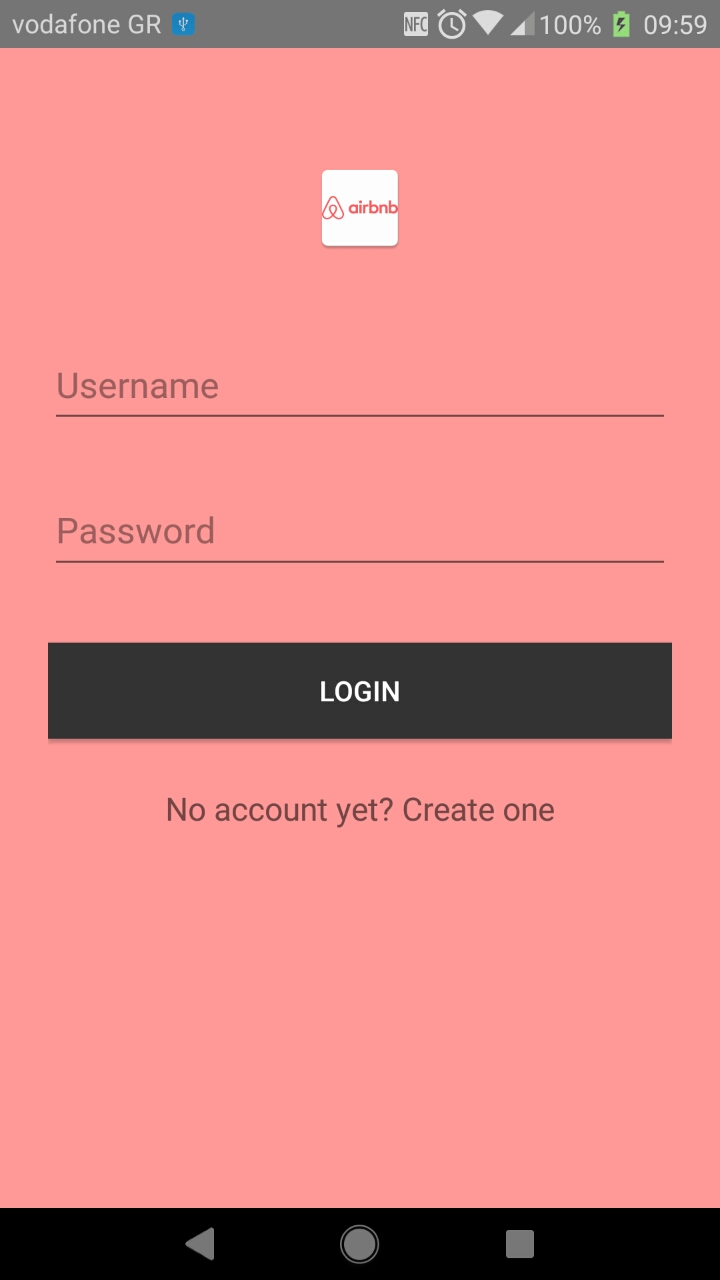
\includegraphics [scale = 0.18] {04-login.jpg}
				\\
			\end{tabular}
			\caption{Register and Login Activity}
		\end{figure}
	\end{center}
	
	\subsection{Home Page}
	
	In this activity, it is checked if the user is logged in. If not, the application redirects them to the Greeting Activity, as mentioned above. SharedPreference values are passed to the HomeActivity's methods onCreate, onResume and onRestart. The BackPressed method restricts the logged in user to go back to the Login screen. Instead it puts the application on the background (minimizes the app). The main content of the HomeActivity is a list of recommendations of residences. with two main toolbars: header (in this case search bar) and footer.
	
	Search bar appears on the top of the Home screen, allowing the user to search on specific residences either by city, dates availability (arrival/departure date), and number of guests. The footer is stable at the bottom of the screen, indicating the main menu of the application (Messages, User Profile, Switch Roles, Logout).
	
	The logic of the recommendations presentation is based on the history of the user, if there is one. More specifically, the \textit{searches table} stores all the city names that the user has searched for. If there are residences related to this city and also satisfy the number of guests and the availability of dates, they appear to the recommendations list. If the user is new, they see the most popular residences based on the reviews being made by other tenants. In any case the residences are sorted based on their average rating. The method implemented for this purpose is the popularRecommendations in the HomeActivity. First of all, a GET request is sent based on the username stored in SharedPreferences so as to get a Users Entity Object. Then, our application checks user's searches and stores them in a HashSet to avoid duplicate cities. For all the cities in the HashSet, we get all the relevant residences and we keep only those that have reviews. For these residences, we store all the reviews in a respective collection.
	
	If the user has not searched anything yet or if there are no residences in the cities searched or if the residences collected have no reviews, we show the user the most popular residences based on their rating. Moreover, we exclude the duplicates and the residences uploaded by the the main logged in user (the host). If, despite all these, the ArrayList of residences is still empty (which means that there are no reviews in our database), a list with all the residences is presented. Finally, the ArrayList is sorted based on the average rating - relevant method is implemented in Residences class, package fromREST (getAverageRating method). In Residences class, a compareTo method, compares two Residences based on their average rating. 
	
	In order to show the results to user, a RecyclerView was implemented. Each list item shows the representative photo of a residence, its price, the city, the title of the residence and the average rating. The Residences Object includes a field named photos, meaning the name of the main residence image which is stored on the server side of the RESTful Service. Through the use of \textit{Picasso} library in the PicassoTrustAll class (we implement the OkHttp so as the https links to work for the images as well), a direct call to the appropriate link of reading the image file is made and appears directly to the ImageView of the list item. An adapter was used so as to create the list items. User can select the residence they like and by clicking on it the ResidenceActivity starts, giving them more details.
	
	It is important to mention here, the way we handle user's navigation either as tenant or user. When they first enter the Home Activity, a boolean variable is used (user), which is passed to all activities upon call, in order to specify the role of the user. The value true means that user is a simple user / possible tenant, while false means that they have changed role into host. This is important, since some activities have a slightly different layout based on user's role, while the home page is completely different between the two roles. Once user chooses to switch role, HostActivity is called and user variable is now false.
	
	\begin{figure} [H]
		\begin{center}
			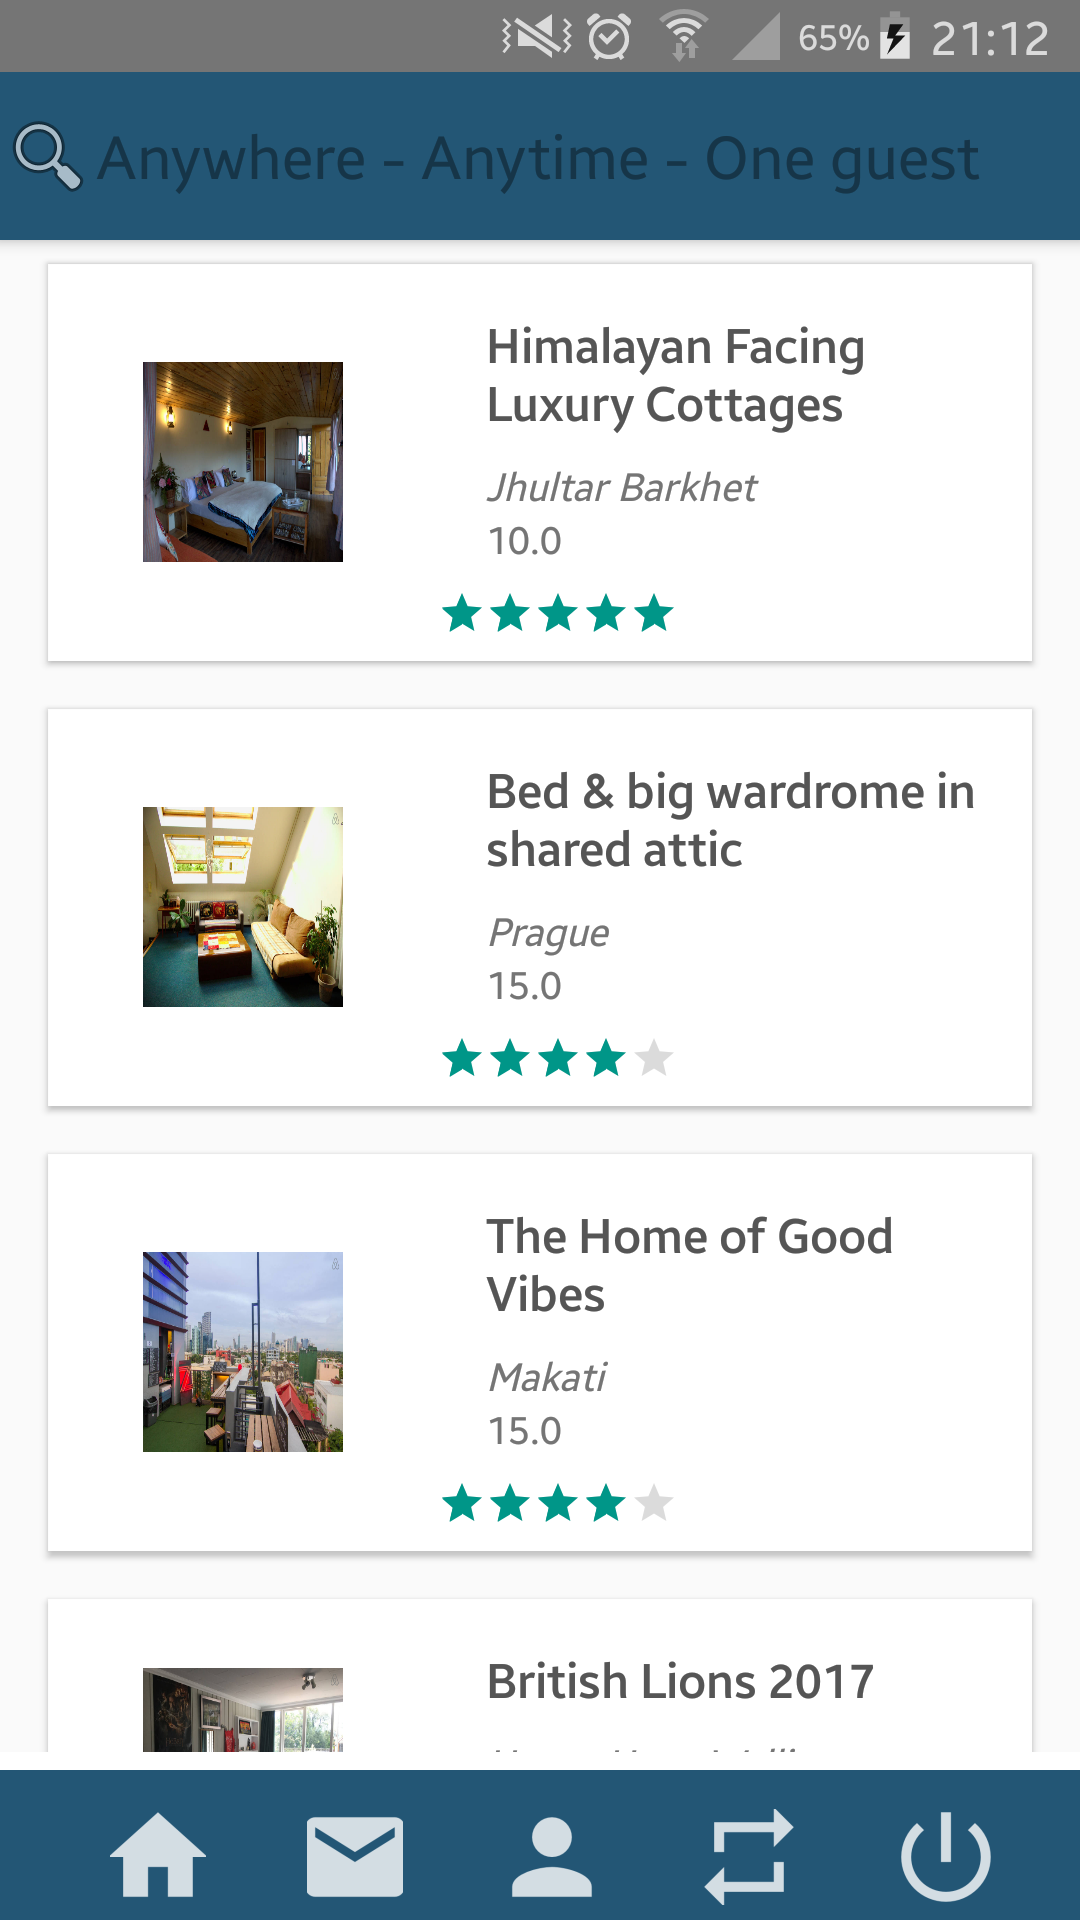
\includegraphics [scale = 0.15] {05-homeActivity.png}\\[1.0 cm]
			\caption{Home Activity}
		\end{center}
	\end{figure}
	
	\subsection{Toolbars}
	
	\subsubsection{Search and Back Toolbar}
	Each Activity contains an upper toolbar and a footer. In the HomeActivity, this toolbar collapses (either on scrolling or clicking the main bar appearing) and the user can fill in the search fields and press the search button. Then, the results are updated in order to comply to the user input. The Home screen reloads and the list is updated. Furthermore, the user can clear and reset all the fields and go back in the initial result.
	
	In all other activities, the upper toolbar has a stable icon on the left, indicating a back button, the title of the activity and usually, another icon on the right, providing access to a popup menu which gives further possibilities to the user. The logic of the back button varies according to the Activity that the user is currently at, as it is not always certain which path was used in order to get there. So in many cases, such as in MessageActivity, HistoryReservationsActivity, or ResidenceActivity, there is a switch case code which reviews the values passed through possible Bundle Objects and decides where to send the user next. This logic is grouped and called also when the user clicks the back button from their device and not only the upper icon. The BackPressed method can't control the variety of these paths by itself, so this custom functionality is very important here. The popup menu existing on some of the activities will be analyzed per case as well as the options provided each time.
	
	\begin{figure}
		\begin{center}
			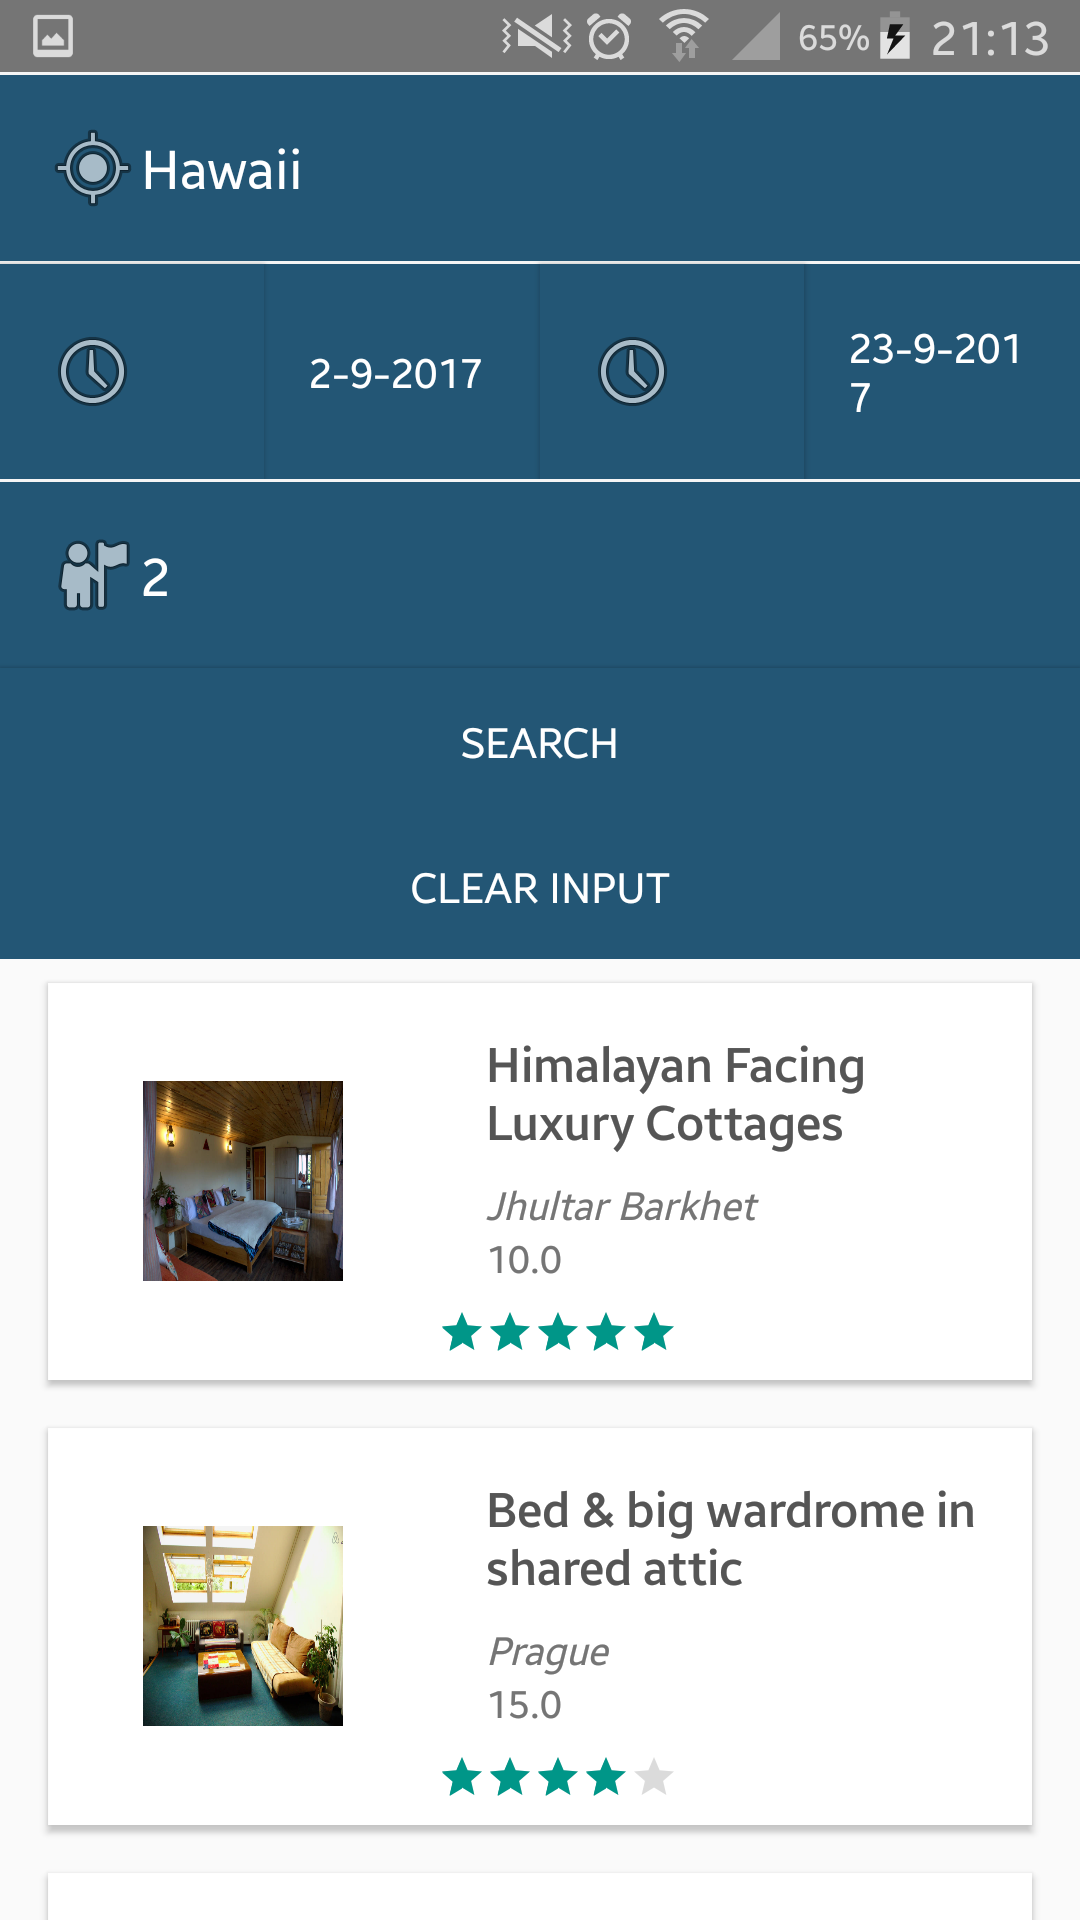
\includegraphics[scale=0.15, keepaspectratio]{06-expandSearch.png}  
			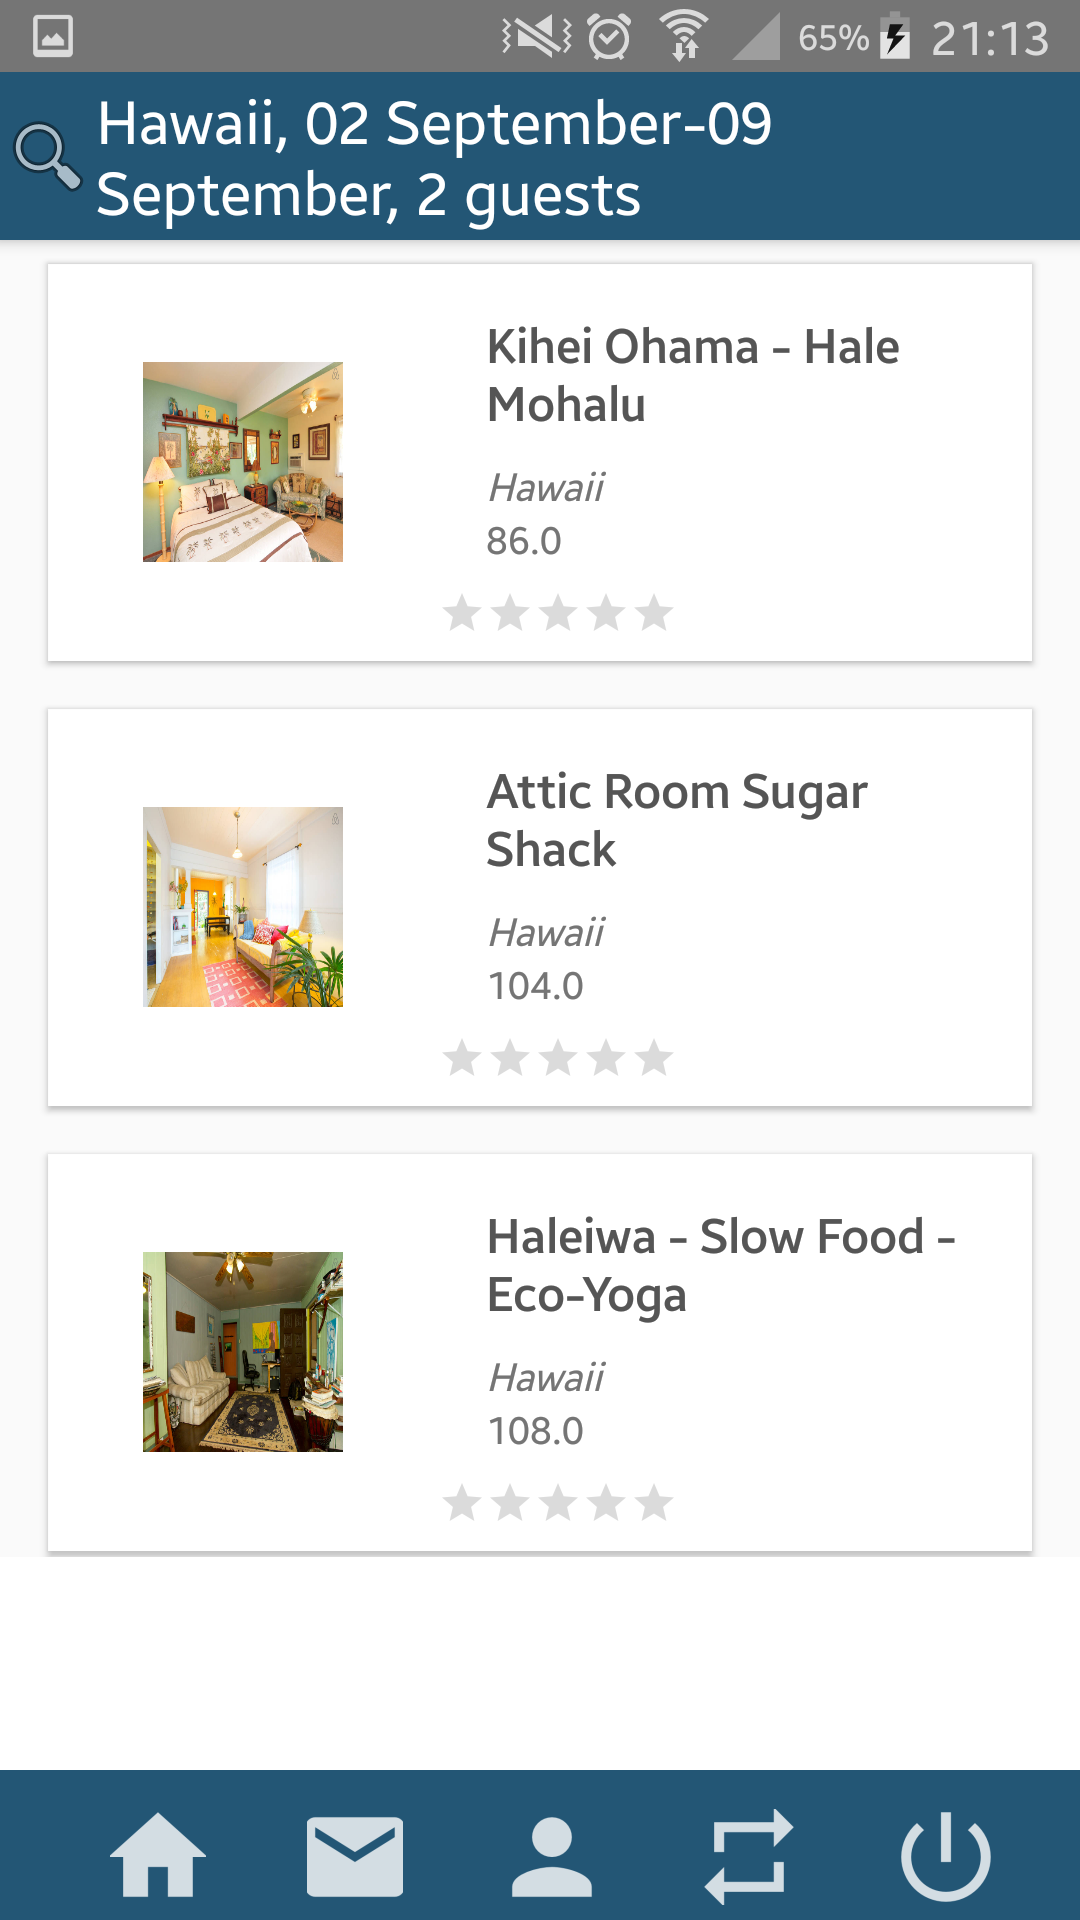
\includegraphics[scale=0.15, keepaspectratio]{07-searchResult.png}  
		\end{center}
		\caption{Expanding search toolbar and search result}
	\end{figure}
	
	\subsubsection{Footer Toolbar}
	The footer toolbar appears in almost all our activities and gives several possibilities to the user. The first image button is used to refresh the home activity. It is checked whether the user is using the application as simple tenant or as a host and the application presents them a different activity (home or host). In case that the user is logged in as tenant, a list of recommendations is presented to him, as described above. Otherwise, the home activity (HostActivity.java) shows a list of all the residences uploaded by the logged in host. The structure of this list is the same, but the options provided there are different and will be discussed later. The second button redirects the user to InboxActivity.java in order to see all the conversations create and messages exchanged. The third option is the profile button in order for the user to manage their personal details. The fourth icon is the switch button which allows them to change role from user to host and the opposite. Finally, the last button allows user to log out from the application. When this button is pressed, the relevant shared preferences are cleared and the user is redirected to GreetingActivity.
	
	\subsection{Detailed presentation of residences}
	The user has access to this activity, by choosing a residence from the list of recommendations (HomeActivity) or their own residences (HostActivity). InboxActivity, HistoryReviewsActivity and HistoryResidenceActivity are additional paths which can navigate the user to the residences screen. At the top bar of the ResidenceActivity, there is the back button calculating to which of the previously mentioned Activities the system will return. A bundle is passed to the ResidenceActivity in order to know which residence the user has chosen and from which activity all the relevant details are and will be presented. 
	
	On the right side of the top toolbar there is the popup icon which gives more options to the user, according to their role. If the user is simple tenant they can see all reviews related to this residence or to view the profile of the host. If the user navigates as host, the menu is different giving him the possibility to view all reservations for the specific residence, view their profile and view all reviews for the residence made by tenants. 
	
	The bottom toolbar of the screen shows the rating and price of the residence. If the user is tenant, a button also appears in order to make a reservation. Otherwise, this button is invisible.
	
	The main content of the residence starts with a slider of images representing details of the residence, for example the house, the view, and anything other the host wants to show. This slider has been implemented through the android library \textit{Android Image Slider} giving the possibility to switch image every few seconds, scrolling horizontally, setting all of them to a specific size of format, giving them title captures and a variety of animations. The main functionality has been set up in ResidenceActivity.java triggering the SliderLayout into activity\_residence.xml. In order for the images to be loaded to the Android app, this library can handle their presentation as long as there is a correct link (external in this case), reading the relevant image file. As used above for Picasso, in the residences list, the same REST call is made here, but with a small difference. The names of the images to be load are extracted from the \textit{images} database table, where there there are saved more than one images to a single residence. If the residence doesn't have any images uploaded, then the SliderLayout is hidden, and the content below appears first.
	
	Below the slider, the user can read some rules, the cancellation policy and the amenities the host provides as well as a short description of the residence. In addition, a map is included in order to present the area where the residence is located. As already mentioned, the address is provided to the rest call. A JSON object is received, from which the specific location is needed (we get the latitude and longitude from JSON object location included in the hole JSON object received). These fields are used in order to create a LatLng object and provide it to map in order to show it (with zoom to this area). We have requested a google key for the use of the map and provided this info in the relevant xml file as well as in the AndroidManifest in order the map to work properly. Also, ResidenceActivity should implement OnMapReadyCallback and override the method onMapReady, where the map is created and zoomed in the residence's location.
	
	Finally, user can see a calendar where min and max dates is the available period given by host (min and max date indicates which dates will be shown in calendar) and also which days are not fully booked. In case the user has already selected dates and number of guests in the search field of HomeActivity, these dates appear as selected on the calendar and the guest's field is automatically completed, otherwise they have to select a start and an end date before proceeding with booking. User can select only two days (a start date and an end date) or they can release a date and pick another one, but in total only two dates can be selected. Before choosing dates the user is asked to also fill the field of number of guests (in case it is empty). The number of guests is required in order to disable some dates that the residence is already fully booked and cannot accommodate the specific guest number. In order to be able to disable some days on the calendar, based on the availability, Caldroid was used (found in git) since the basic calendar did not have such choice.
	
	\begin{center}
		\begin{figure}
			\begin{tabular}{c c c }
				
				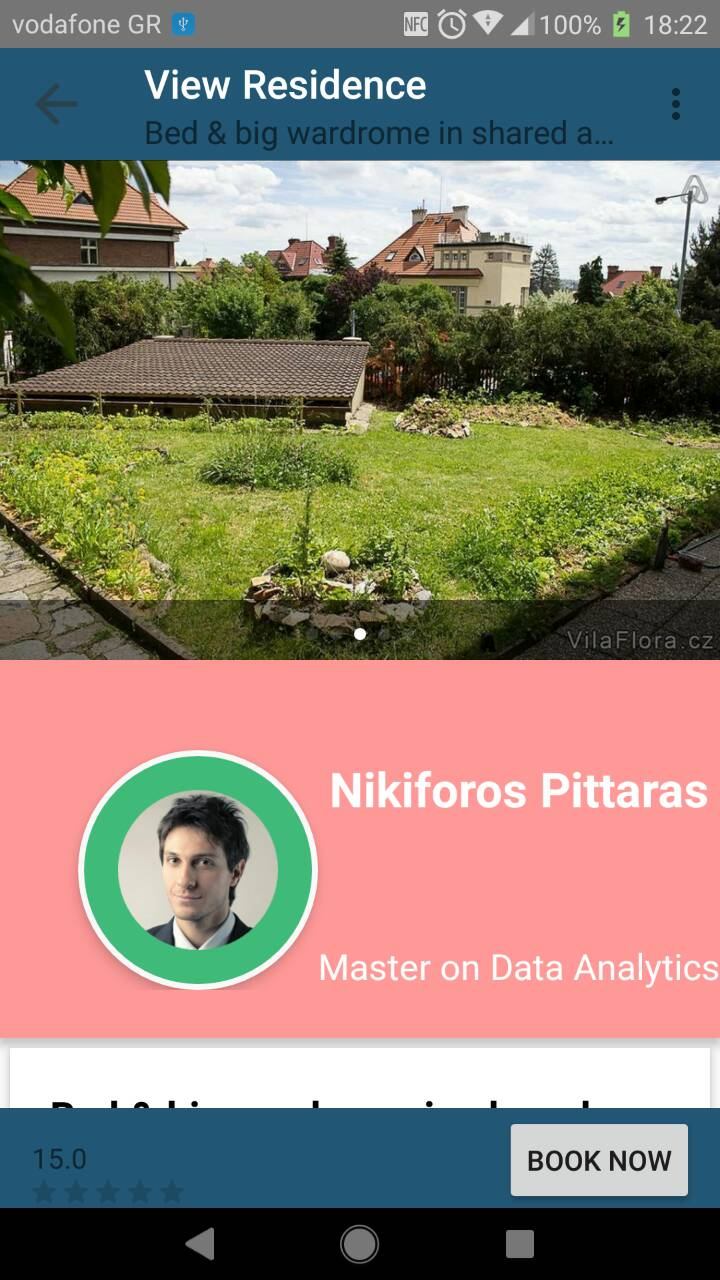
\includegraphics[scale=0.18, keepaspectratio]{slider.jpg}  
				&
				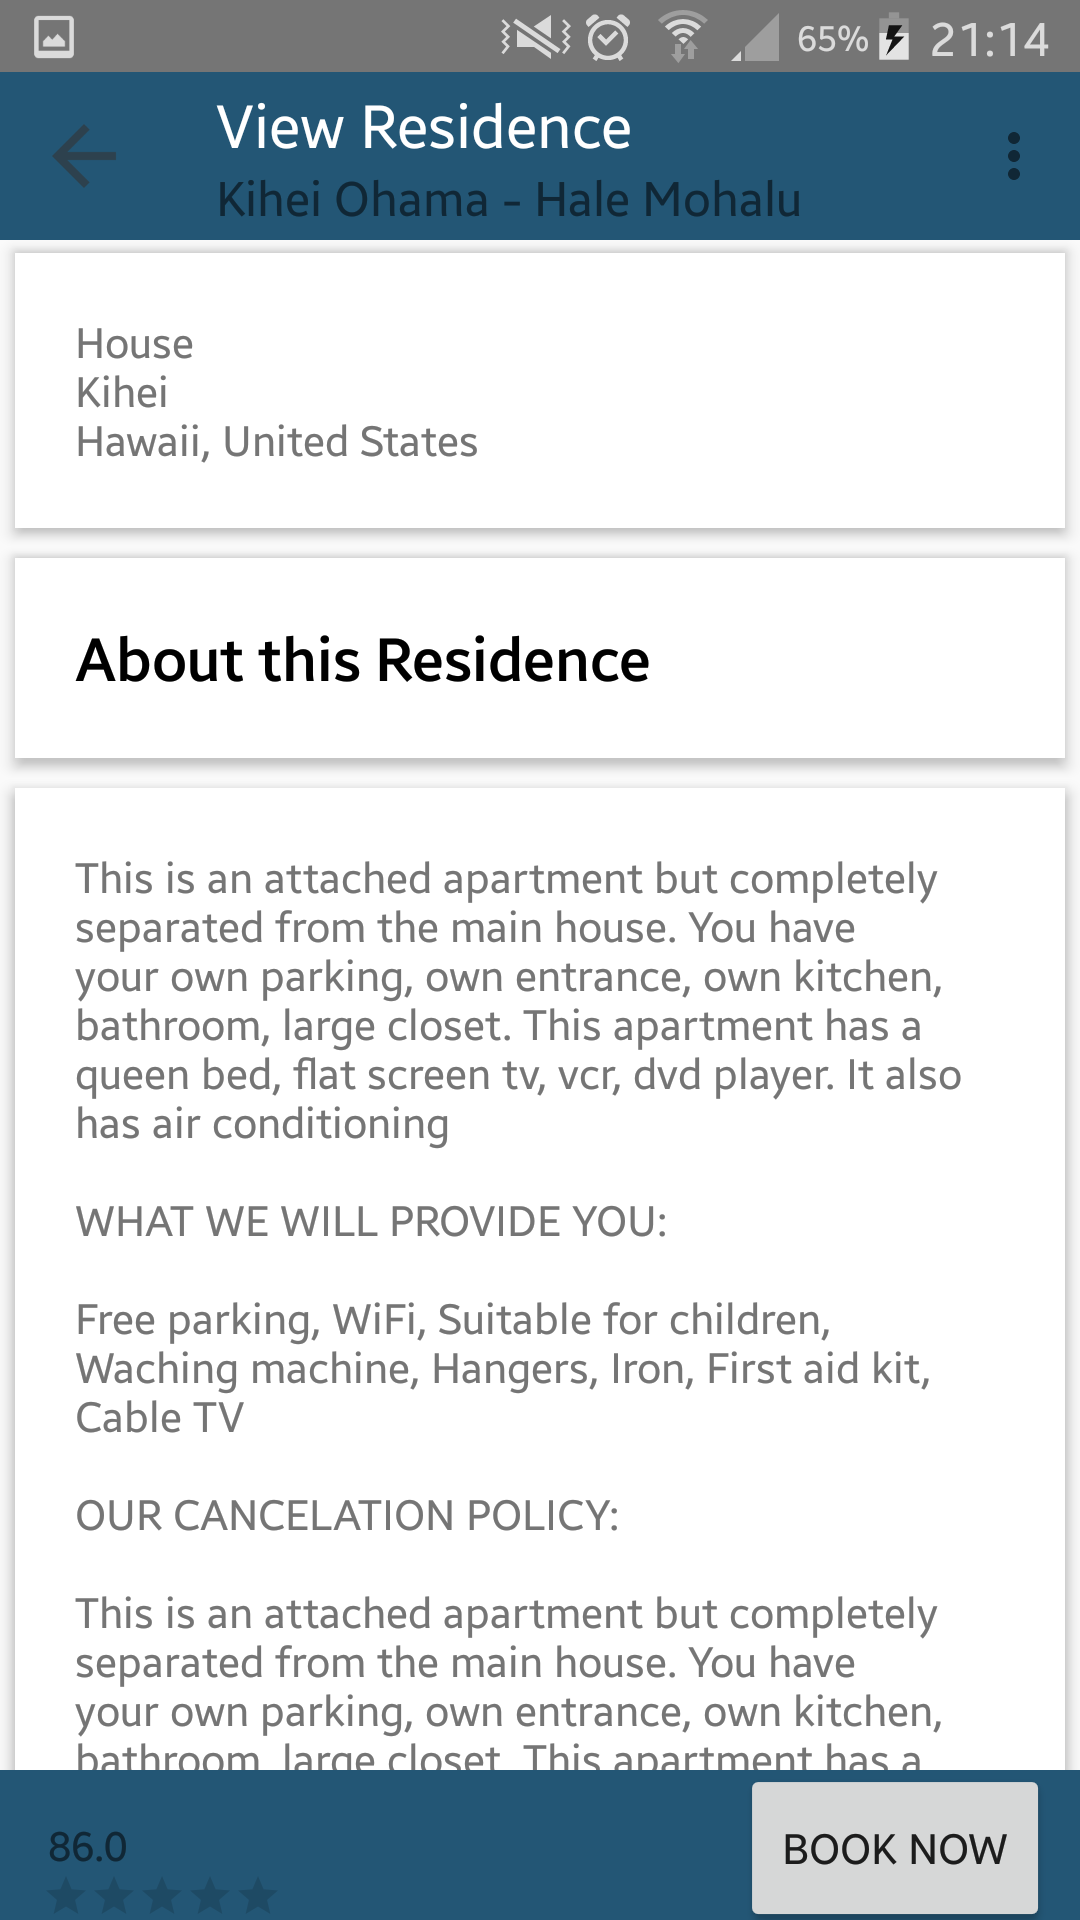
\includegraphics[scale=0.12, keepaspectratio]{08-Residence01.png}  
				&
				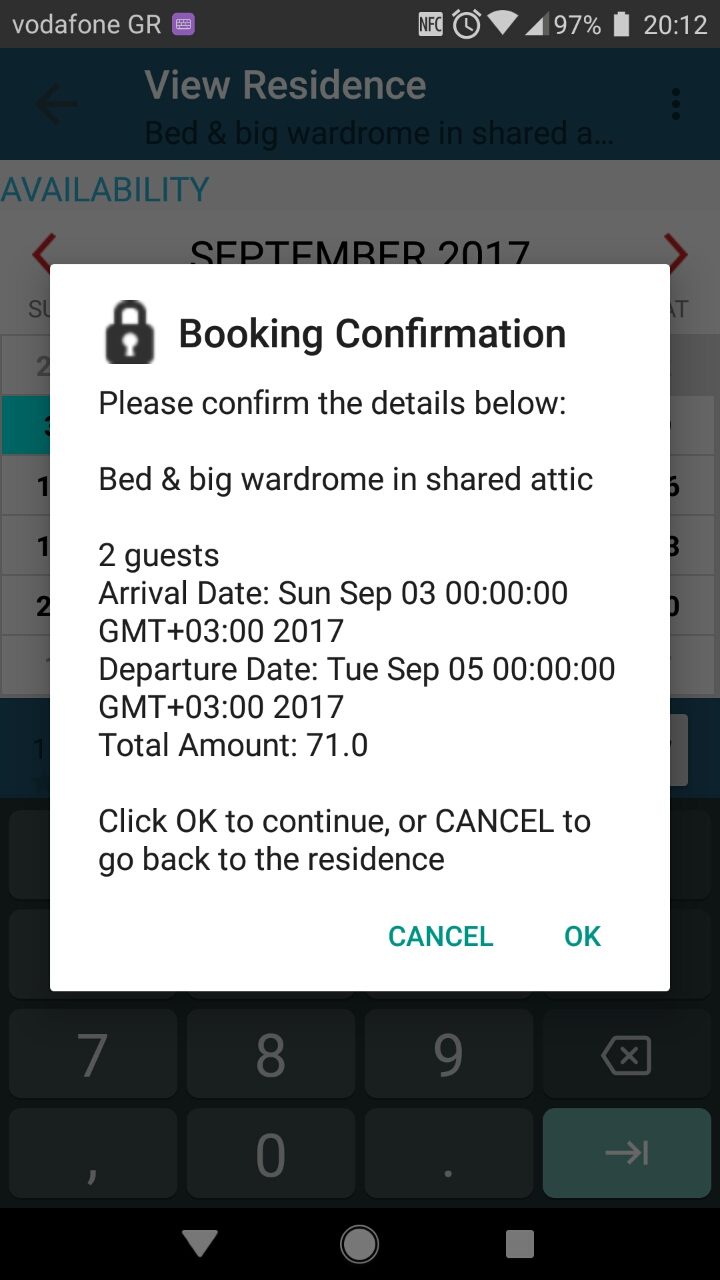
\includegraphics[scale=0.18, keepaspectratio]{11-bookConfirm.jpg}
				\\
			\end{tabular}
			\caption{Residence Activity}
		\end{figure}
	\end{center}
	
	\begin{figure}
		\begin{center}
			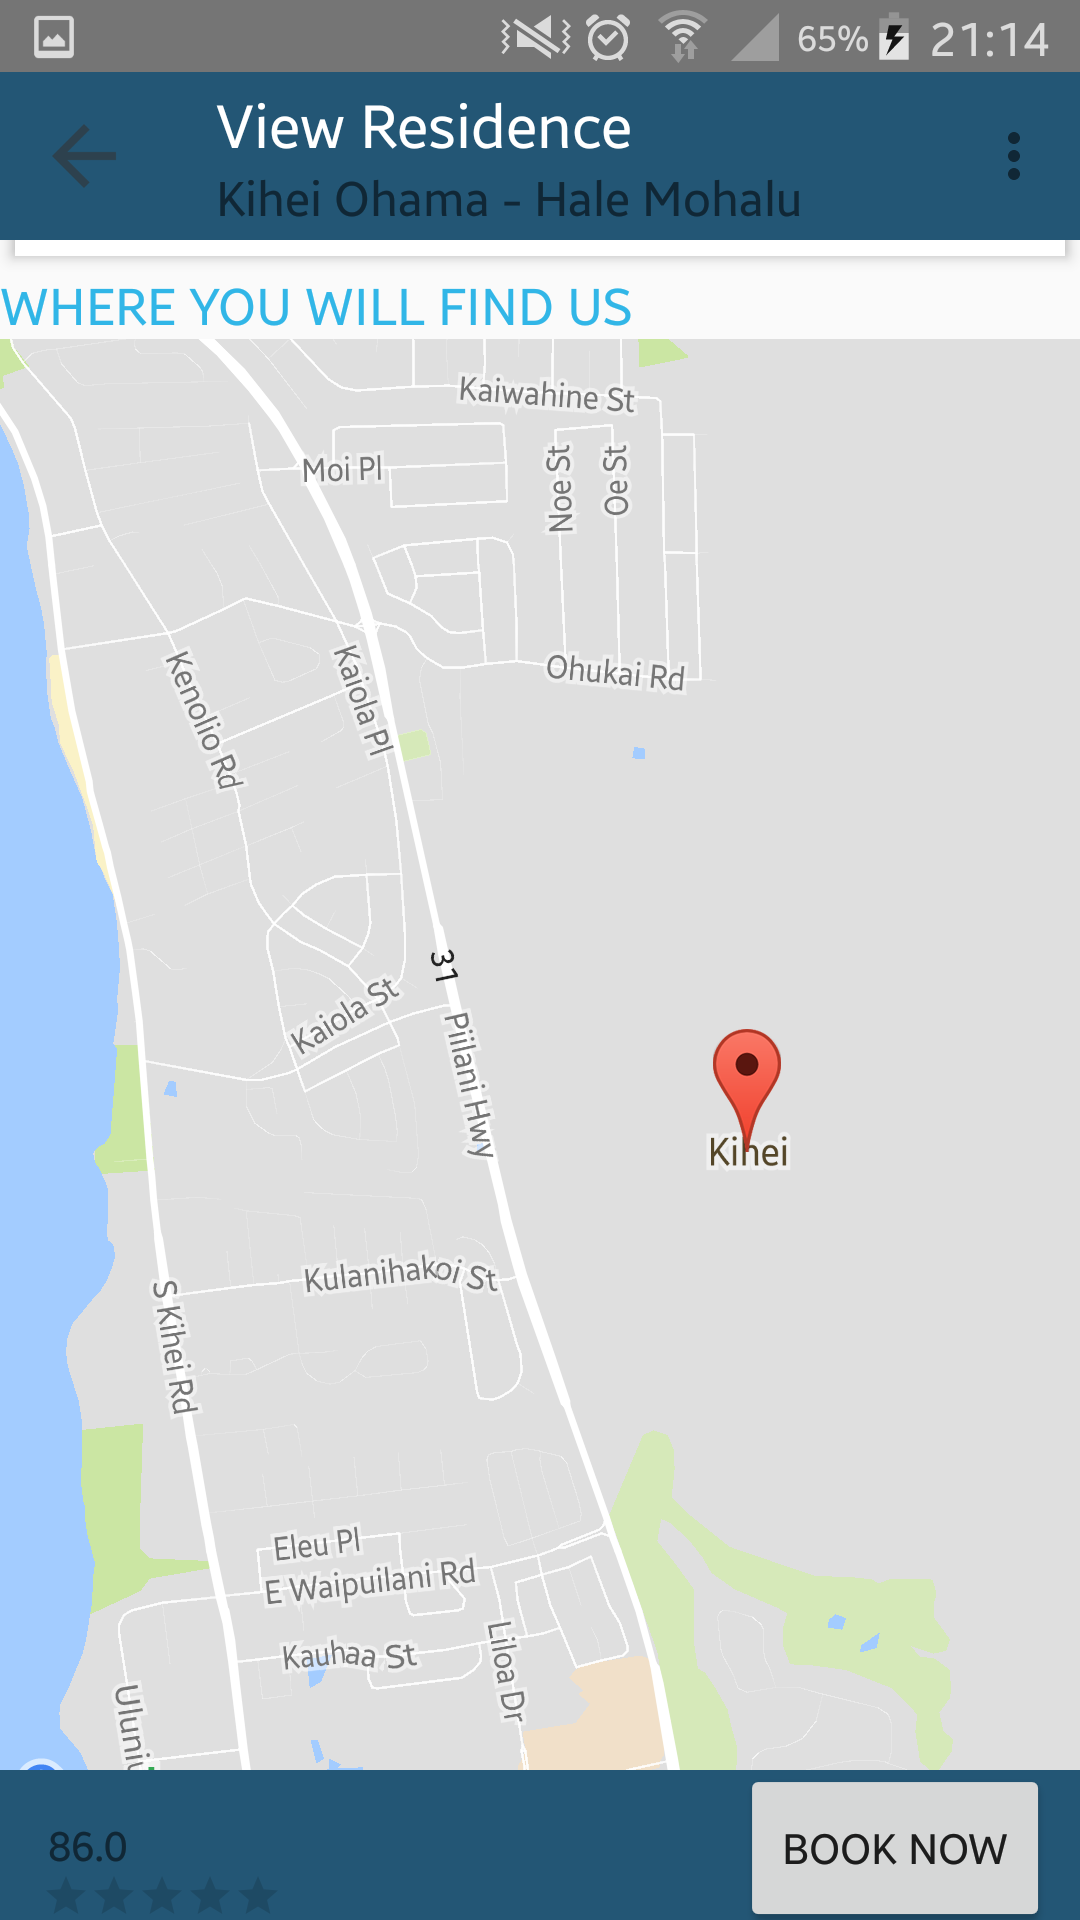
\includegraphics[scale=0.12, keepaspectratio]{09-Residence02.png} 
			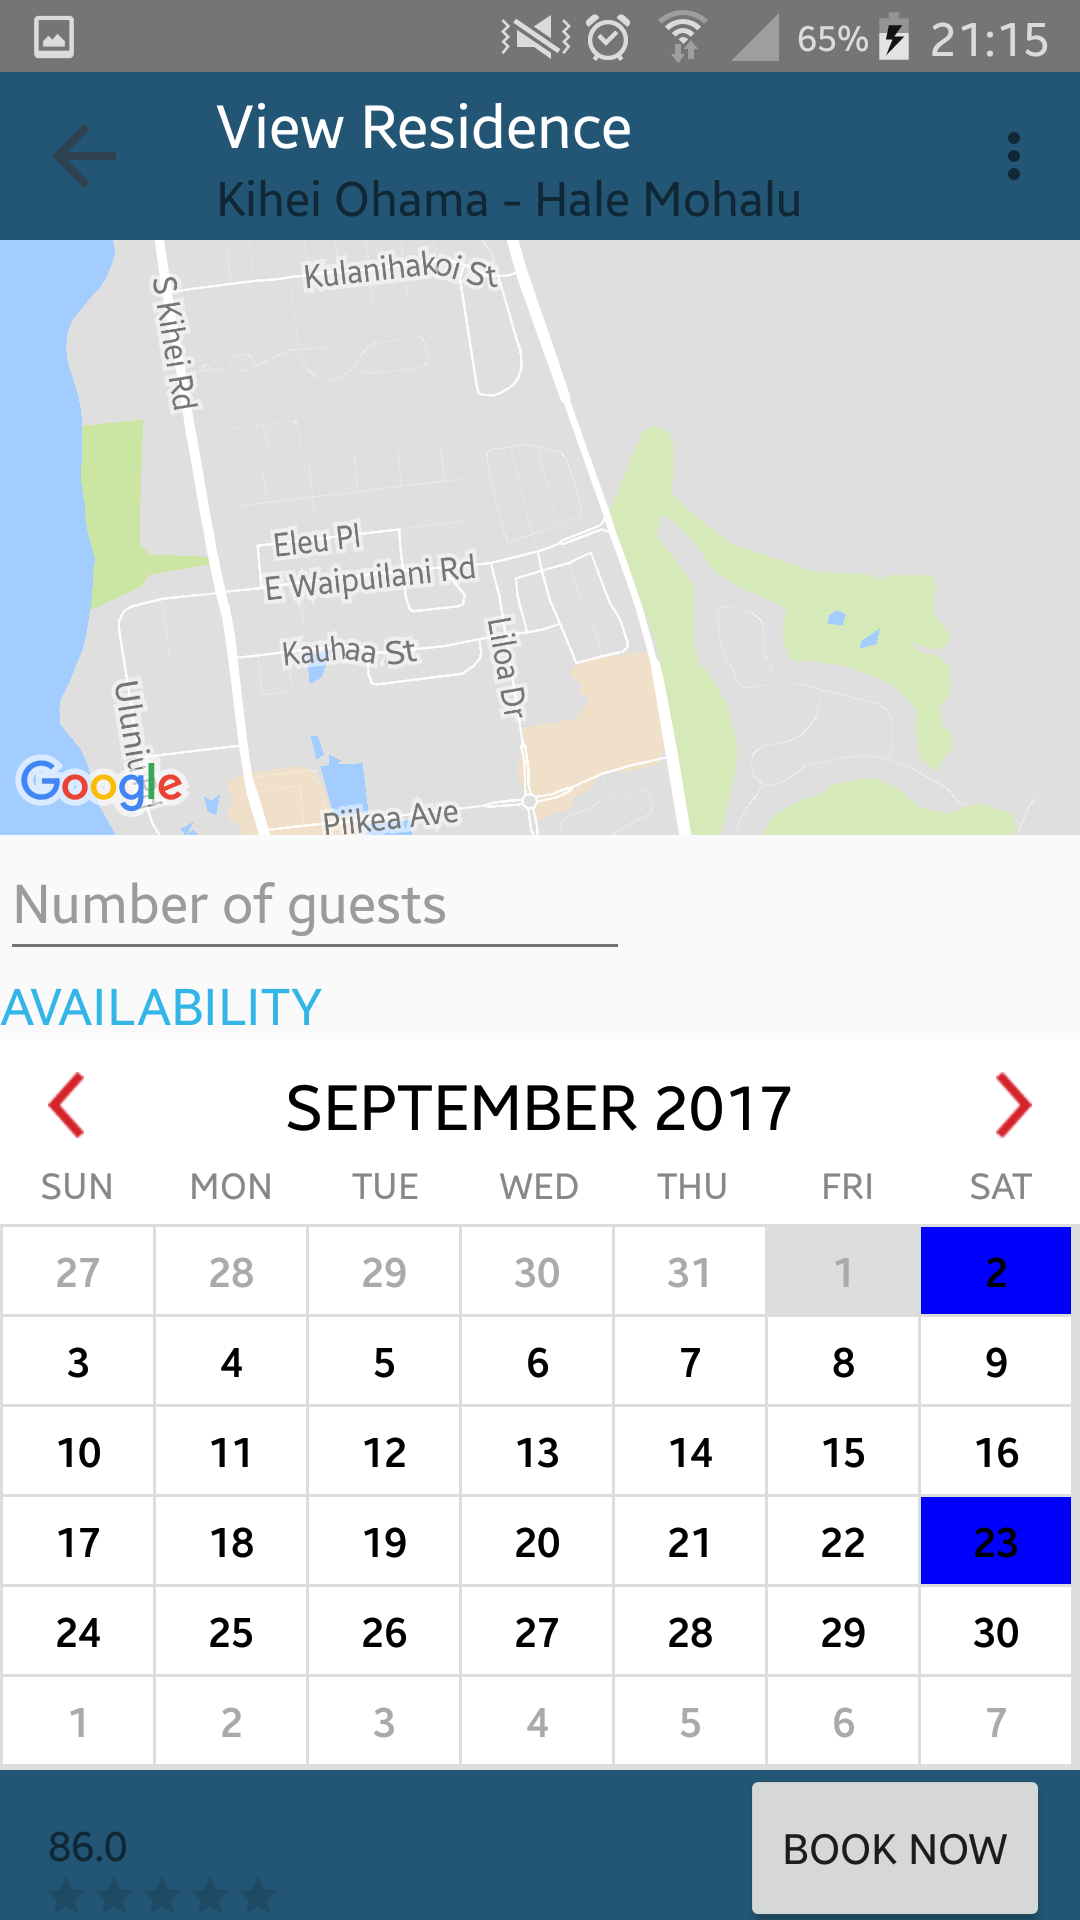
\includegraphics[scale=0.12, keepaspectratio]{10-Residence03.png} 
		\end{center}
		\caption{Map and Calendar in Residence Activity}
	\end{figure}
	
	\subsection{Inbox}
	
	\subsubsection{Conversations}
	When the Inbox button is clicked, the \textit{ConversationsActivity} is triggered, and the user is redirected to a list of all the conversations that are related to them. The main database table used is the \textit{conversations} table which is accessible through the \textit{Conversations.java} Entity Object from the fromRESTful android folder. The user is not able to create a new conversation from there as this is only available through the profile of the either the host or tenant on each case. The Activity is connected to the activity\_inbox.xml file where a RecyclerView adapter is initialized passing the ArrayList of Conversations to the specific format. Each recycler item shows the subject name (which is already assigned from the title of the related residence at the beginning of the conversation), and the name of the other user. As the conversations table stores the sender and receiver user id in the database (based on who started the conversation the first time) the name of the user in the recycler item changes according to which one of the two is currently logged in. So the logged in user will always see the name of the other that they communicate with. 
	
	The fields \textit{read\_from\_sender} and \textit{read\_from\_receiver} are depending to the \textit{messages} table where the system counts the number of unread messages for the specific conversation. If the number is higher than zero(0) for the sender (or respectively the receiver) then the recycler item in the inbox will appear with bold letters indicating that it isn't opened yet. Once the user clicks onto an item they are redirected to the messages screen. At this moment the database is updated (with a @PUT call) and the \textit{read\_from\_sender} (or respectively \textit{read\_from\_receiver}) field updates its' value to one(1). 
	
	On a prolonged click on a conversation item, a ContextMenu is initialized and several options appear. First there is the \textit{Open Message}, which is the same action as on a single click, that open the messages chat screen. Then there is the \textit{View Residence} action which redirects the user to the screen of the residence that is related to the conversation. Last there is the \textit{Delete} action where the user has the ability to delete the conversation. Once clicking this option a confirmation message appears asking the user if they are sure they want to continue. After accepting, conversations screen reloads and the specific item doesn't exist anymore. In this case, the conversation isn't totally deleted from the database as it must still be enabled for the other user to see. That means that if the sender deleted the message, the receiver should still be able to see it. On the contrary, the deleted\_from\_sender (or respectively deleted\_from\_receiver) field is updated, setting its' value to one(1). When this happens, this conversation is only visible to the user that has its' value to zero(0).
	
	\begin{figure} [H]
		\begin{center}
			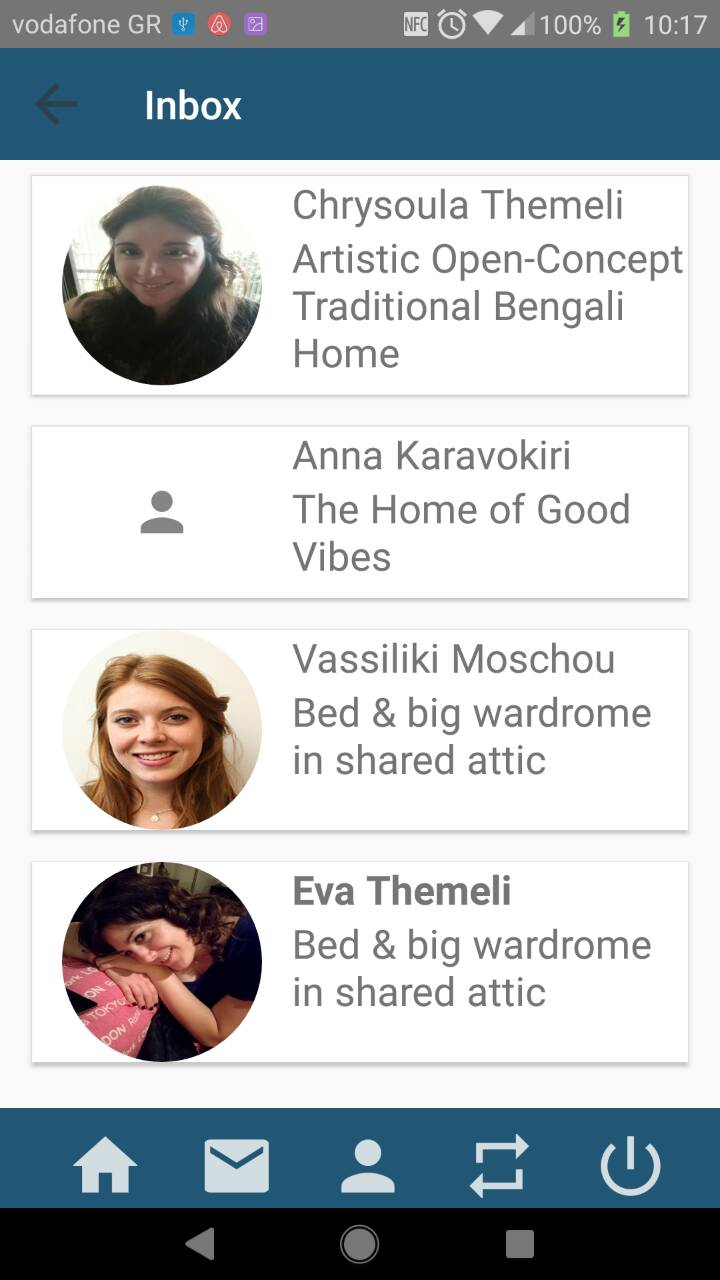
\includegraphics [scale = 0.18] {12-inbox.jpg}\\[1.0 cm]
			\caption{Inbox Activity}
		\end{center}
	\end{figure}
	
	\subsubsection{Messages}
	In order to show the messages of a conversation, we have used a RecyclerView and for each item we show the username (with bold), the body of the message and the date sent (MessageActivity.java is used and activity\_message.xml as the main layout). For the layout, we have used a chat layout, the messages sent by the logged in user have grey background and aligned to the right while the replies are with blue background and aligned to the left. For each message, we check who is the sender in combination with the currently logged in user in order to adapt the layout correctly. On top of the recycler layout there is the subject of the conversation as triggered from the conversation\_id contained in every message. 
	
	In order to know if we have to update an existed conversation with new messages, or create a new  one, there is a check happening  depending from where the user opened the messages screen. The Bundle values being transferred indicate whether there is a specific conversation id, that the new message shall be assigned to - this means that the user opened the chat from the inbox list. Otherwise, there must be a residence\_id value which will help search the conversations\_table, in combination with the sender/receiver ids.  If no conversation found, then a new @POST call occurs, creating a new conversation with the residence\_id and the subject (residence title) of the Bundle values, plus the user ids of the current logged in user and the host of the residence. After a successful creation of the conversation, the same criteria is used in order to get the conversation\_id, and after all, a @POST call is made on the RESTful Service creating a new row on the messages\_table. In the same time there is a value \textit{isNewMessage} from the side of android indicating which of the above will occur.
	
	The user can long click on every message item of the chat and a ContextMenu window will popup giving them the ability of two actions. The first is to \textit{delete} one specific message. Again as before, this message won't be deleted permanently but the value deleted\_from\_sender or deleted\_from\_receiver will be updated to one(1). In order to understand if the user that wants to delete the message is the sender or the receiver, the system goes back to the conversation entity and checks the ids that have been set as sender and receiver. With this way there is a proper connection between the two tables keeping the main functionality clear. The second option is to \textit{copy} the specific message. This is useful if the user wants to paste it together with the new message content that they are going to send.
	
	Below the recycler list there is an EditText field where the user can write a new message, and press the send icon button to send it. At this moment, the messages screen is reloaded with the new message added to the chat layout, and a Toast notice appears saying that the message was sent. From the moment the user sends a new message, if he is the sender, the field of the related conversation read\_from\_receiver goes to zero(0) as read\_from\_sender is one(1). The delete statuses for both the sender and the receiver go back to zero(0) no matter what their value was before, as the conversation is activated again. 
	
	\begin{figure} [H]
		\begin{center}
			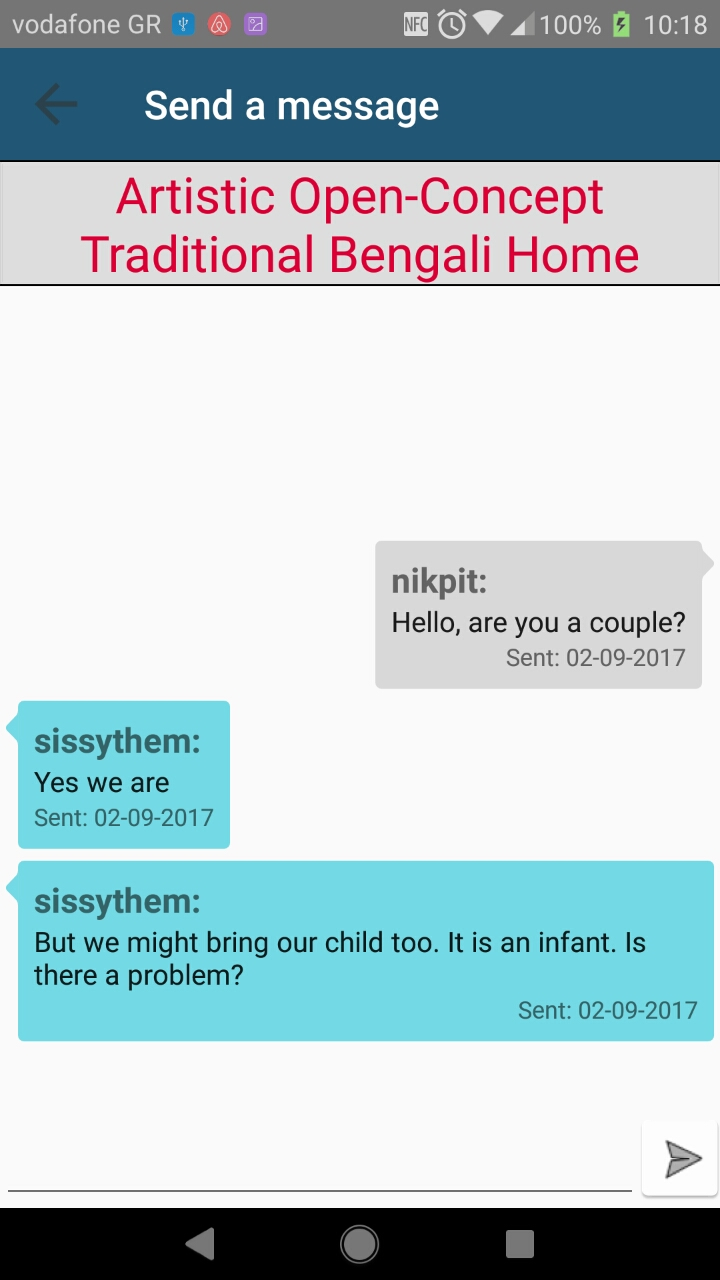
\includegraphics [scale = 0.18] {13-message.jpg}\\[1.0 cm]
			\caption{Message Activity}
		\end{center}
	\end{figure}
	
	\subsection{Reviews}
	
	By selecting the Reviews (\textit{ReviewsActivity}) option at the popup menu in the ResidenceActivity, a new activity starts where all posted reviews for this residence appear. A ListView is used and each item has user's profile photo, the username and the comment. At the bottom of the activity, if user has already made a reservation (and the period of this reservation is in the past), an edit text appears in order to leave a comment, a rating bar and a button to post the comment and the rating. In case user has never made a reservation to the specific residence all these three fields (EditText, RatingBar and Button) are invisible. 
	
	In addition, a similar activity is created and is accessible from ProfileActivity. When user chooses the button profile from the footer toolbar, he can view his profile. At the upper toolbar, there is a button, which when pressed a pop up menu appears and user can view all the reviews he has posted, with the same layout as above. When \textit{HistoryReviewsActivity} is accessed, user reads all his reviews and he can also select by pressing a review to either view the residence or contact the host or delete his review.
	
	\begin{center}
		\begin{figure}
			\begin{tabular}{c c c}
				
				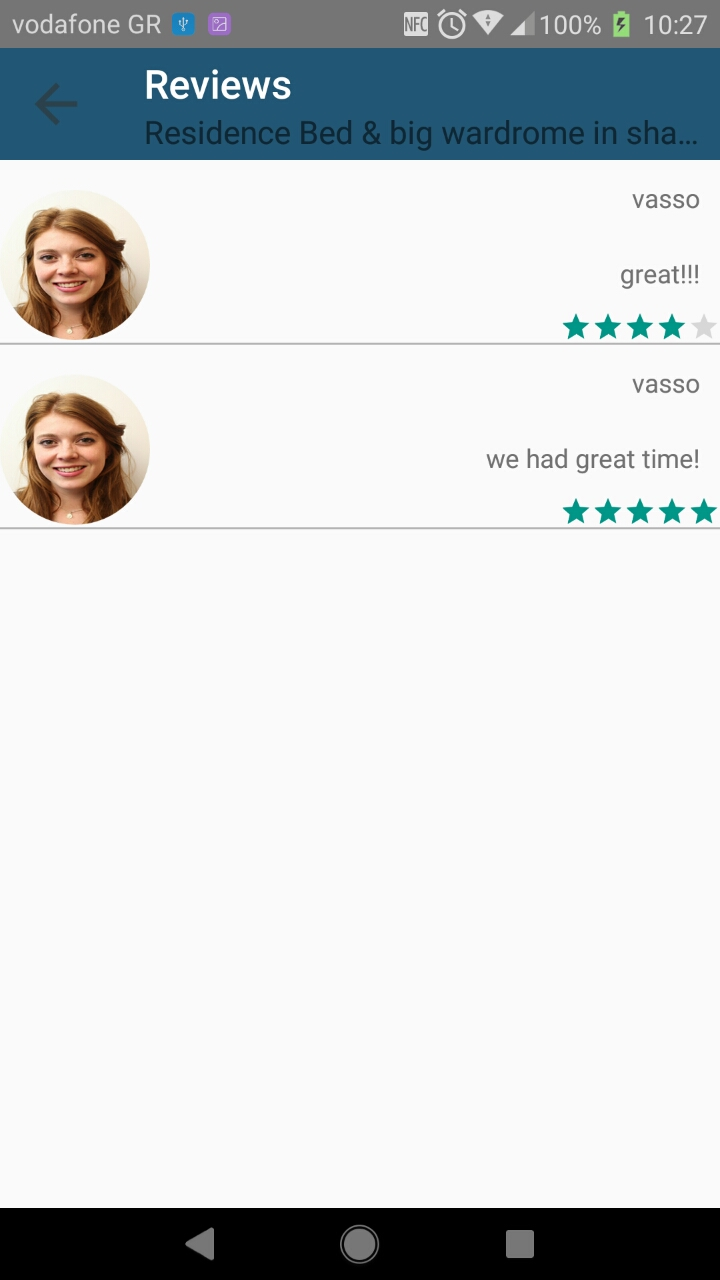
\includegraphics[scale=0.16, keepaspectratio]{14-reviews.jpg}  
				&
				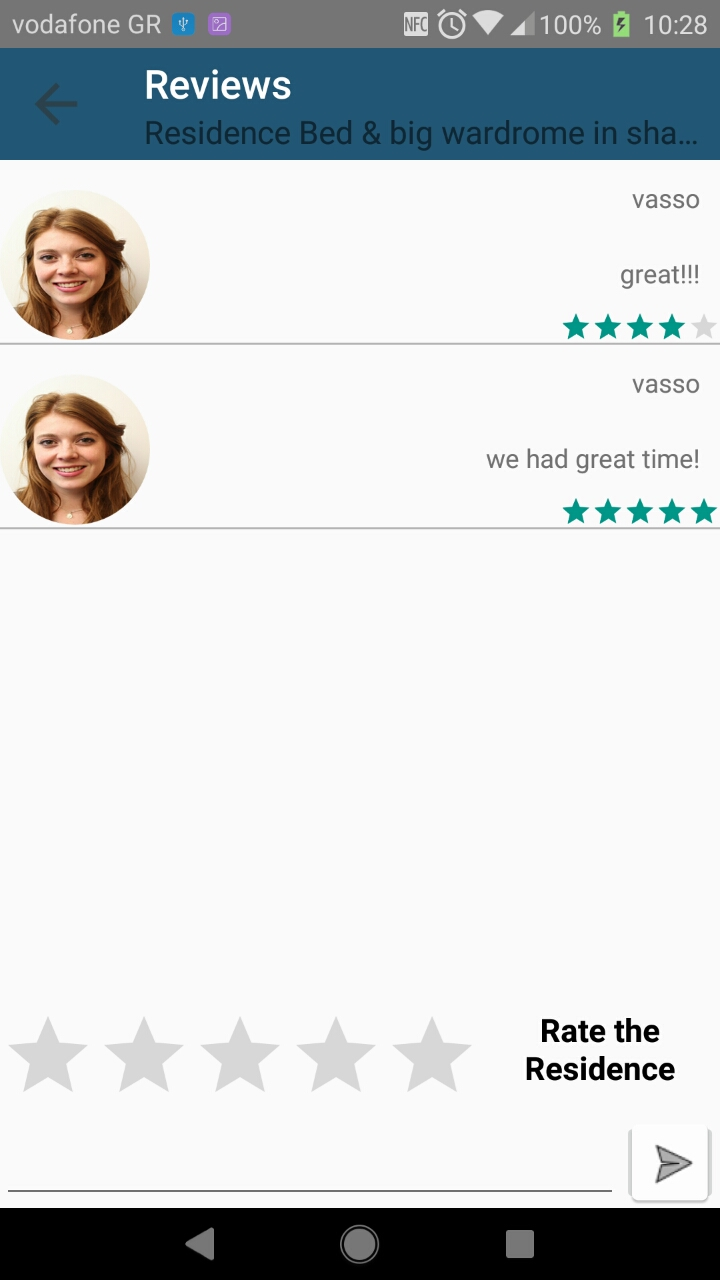
\includegraphics[scale=0.16, keepaspectratio]{15-reviews.jpg}  
				&
				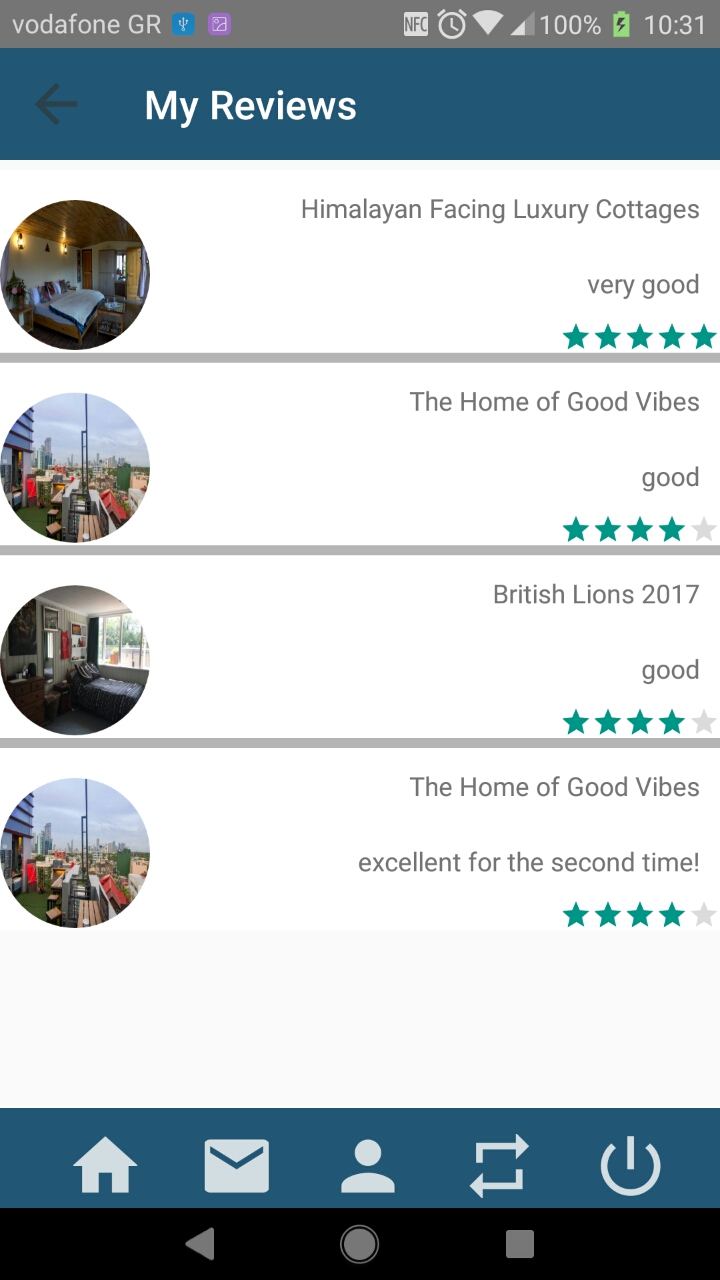
\includegraphics[scale=0.16, keepaspectratio]{16-historyreviews.jpg}
				\\
			\end{tabular}
			\caption{Reviews and HistoryReviews Activity}
		\end{figure}
	\end{center}
	
	\subsection{User profile}
	As mentioned above, the user can select to enter to other activities using the footer and one option is to navigate to his profile. When the related button is pressed, a new activity appears, the ProfileActivity. In this activity user can see his profile photo, his name, last name, username  and every other user field stored in the database. A toolbar is used in the upper side of the activity giving user the possibility to go back, or choosing an action from a popup menu. From the popup menu they can choose to view a history of their reviews, reservations and to edit or delete their account. Below there is a presentation of the menu options.
	In order to display the profile picture of the user in ProfileActivity and all other activities that the profile picture appears, we have implemented the CircleTransform class, in order to crop the profile image in a cycle and fit the layout of the relevant ImageView. 
	
	\begin{center}
		\begin{figure}
			\begin{tabular}{c c c}
				
				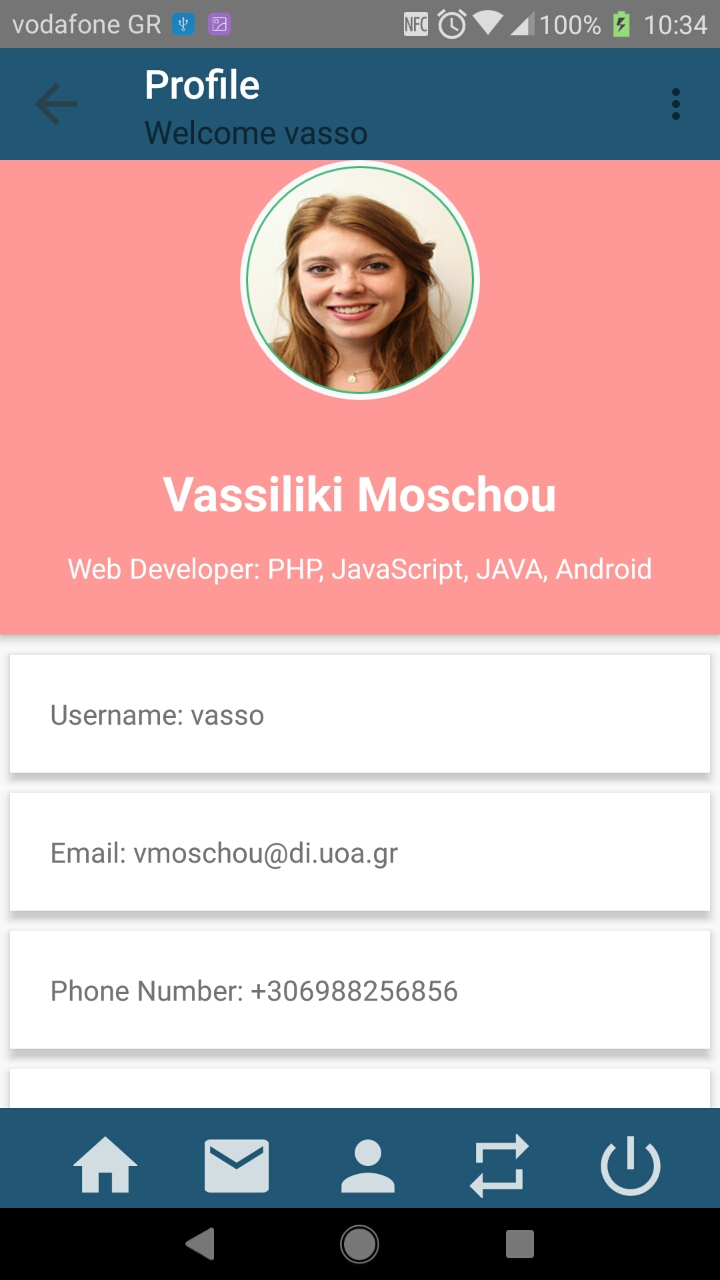
\includegraphics[scale=0.17, keepaspectratio]{17-profile.jpg}  
				&
				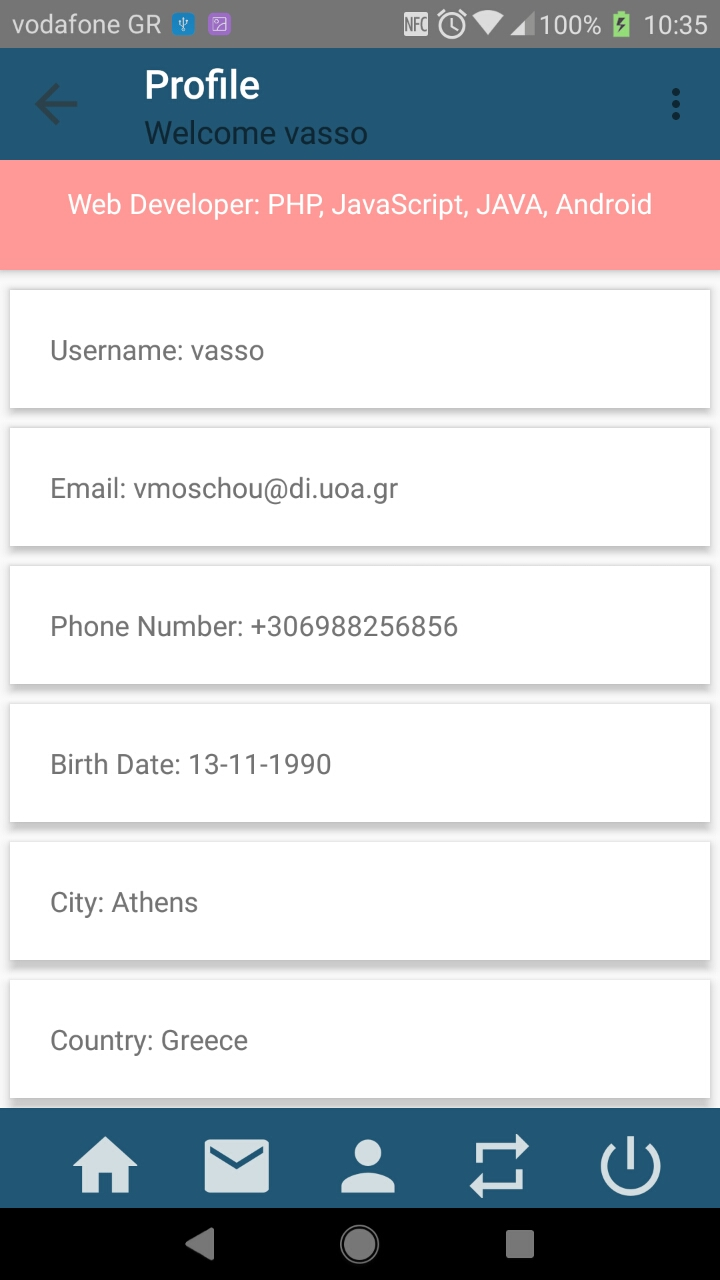
\includegraphics[scale=0.17, keepaspectratio]{18-profile.jpg}  
				&
				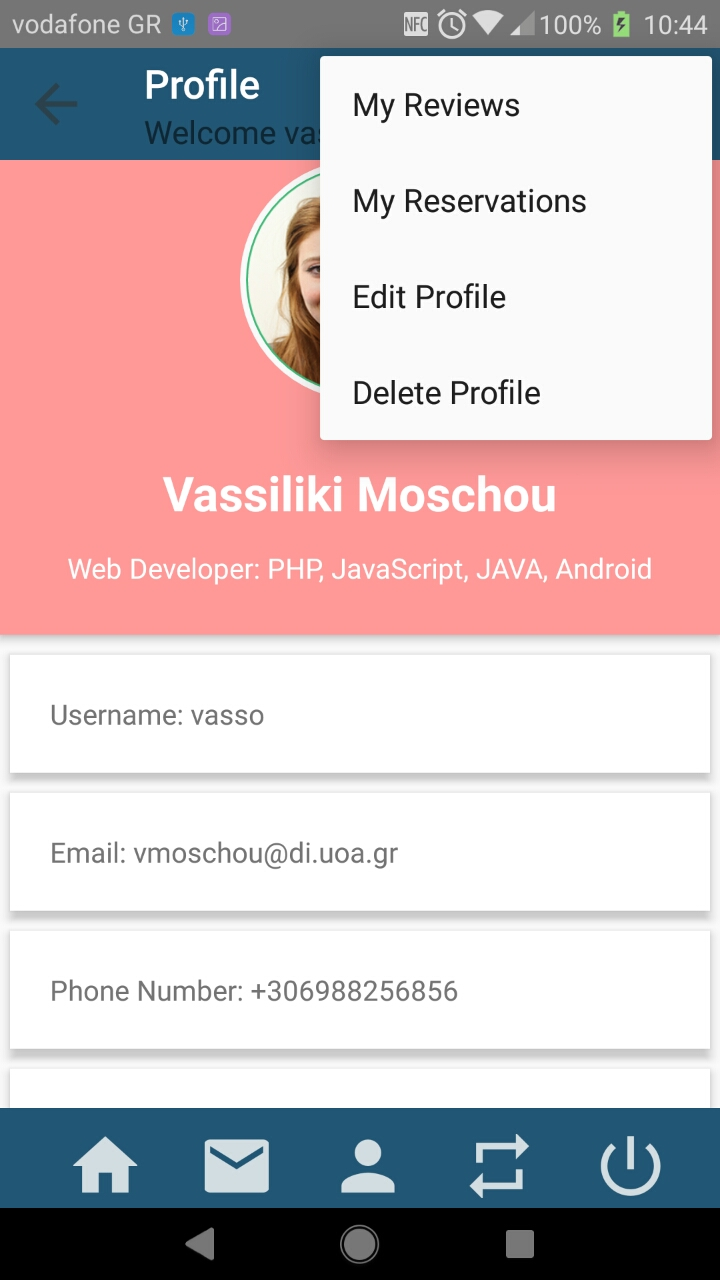
\includegraphics[scale=0.17, keepaspectratio]{19-profile.jpg}
				\\
			\end{tabular}
			\caption{Profile Activity}
		\end{figure}
	\end{center}
	
	\subsubsection{View Review's History}
	Although this activity is described in the Reviews subsection, we will summarize its functionality here:
	In this activity, user can see all reviews he has performed and by pressing each list item the ResidenceActivity starts in order to present respective residence. All reviews are presented using a ListView layout and each item shows the profile picture of the user, his username, the comment and the rating. Also, following the same logic, we use a toolbar with a back button and the title of this activity, as well as a footer toolbar with the usual buttons (home, inbox, profile, switch role and logout). Furthermore, user can select a review and a context menu will appear giving him the possibility to delete it, contact the host or view respective residence.
	
	
	\subsubsection{View Reservation's History}
	In a similar logic, our application presents to user all the reservations that they have performed and have the choice to view each residence by clicking an item from the list. In addition to that, user can cancel their reservation if the period of the booking is in the future or contact the host. In case that user navigates as host, he can contact the user who has performed the reservation of his residence.
	
	Here, we have selected to present the reservation with a RecyclerView showing for each item the title of the residence, its location and the period booked.
	
	\begin{figure} [H]
		\begin{center}
			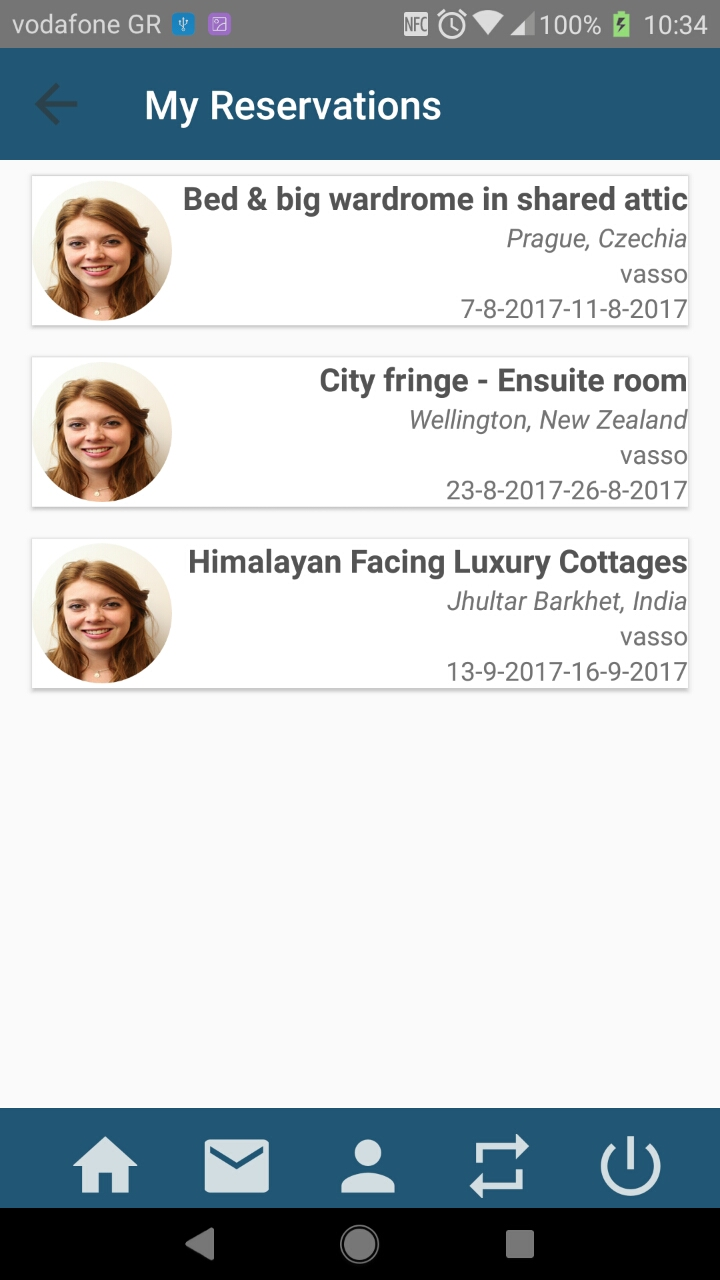
\includegraphics [scale = 0.18] {20-reservations.jpg}
			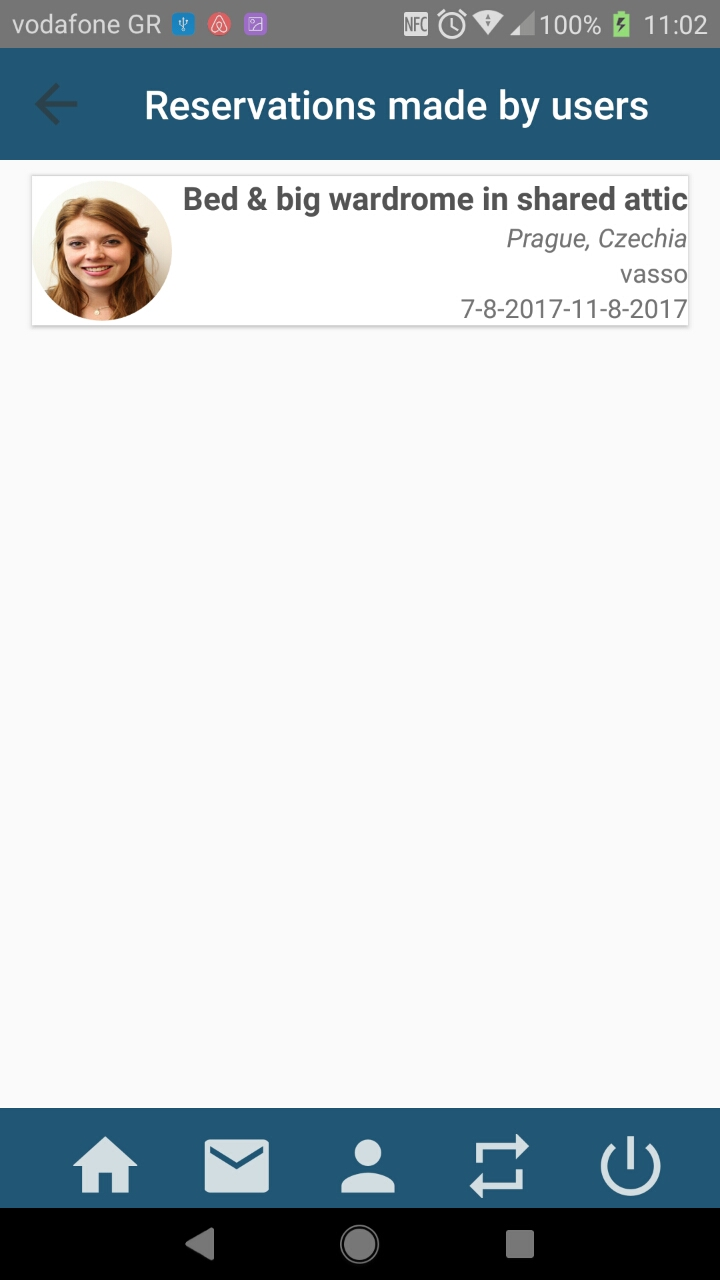
\includegraphics [scale = 0.18] {24-reservationsByUsers.jpg}
			\caption{History Reservations Activity}
		\end{center}
	\end{figure}
	
	\subsubsection{Edit Profile}
	By pressing the edit profile option, a new activity starts (\textit{EditProfileActivity.java}) presenting all user information and giving the possibility to update these details. User can edit all the fields of his profile, except his username. However, for the email field, we check if the email is used by another user. In case the email being new or being the same as before, we set the boolean variable emailIsNew as true, otherwise as false. Only in case it is true we let the user to proceed and save the changes. 
	
	The first item on the screen to edit is the profile photo. The user is also able to upload a profile photo for their account. When clicking on the Button \textit{uploadImage}, the device's gallery app gets triggered and the user has to ability to choose a single image from all of their local device folders. 
	
	After finishing the personal details processing, together with the image selection, user presses the save button and a PUT request is sent in order the database to be updated. After a successful update, a second call is happening in order to save the image file to the server. Thanks to retrofit, the request being sent from android has a @Multipart annotation sending together with the @Header token, the RequestBody and MultipartBody file parameters that conclude the structure of the image file. The RESTful Service from the other side, using the jersey library, understands the annotation by taking as parameters a @FormDataParam InputStream and FormDataContentDisposition types of values. The path of storing the photo is declared on the REST side and a custom name is created for the image. The field \textit{photo} in users table of the specific user gets updated through query call, and the response is the name of this image. If no image is uploaded or there was a failure on the process, no photo is shown and only a default user icon appears on the screen. If the user wants to edit again their profile and selects a different image to upload, the previous one will be replaced and deleted too from the server folder. After a successful edit, the system redirects the user back to the ProfileActivity with the photo and all the fields updated correctly.
	
	\begin{figure} [H]
		\begin{center}
			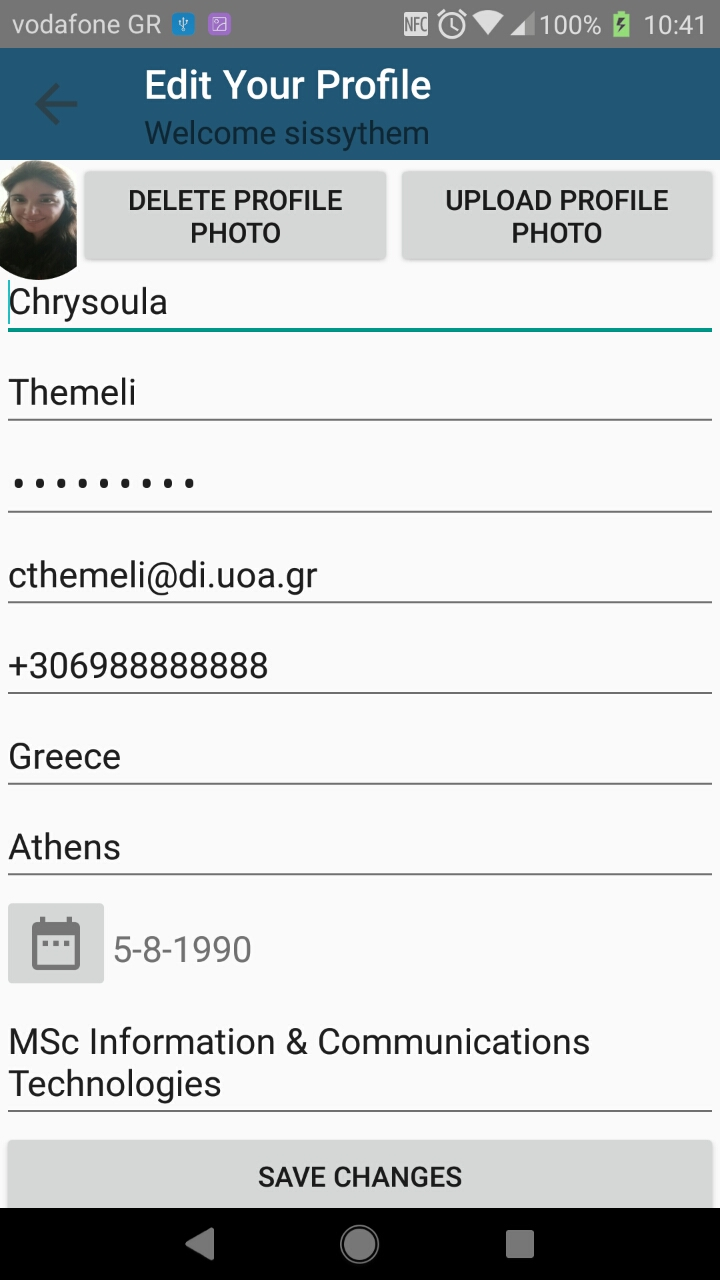
\includegraphics [scale = 0.18] {21-editProfile.jpg}\\[1.0 cm]
			\caption{Edit Profile Activity}
		\end{center}
	\end{figure}
	
	\subsubsection{Delete Profile}
	Finally, we also let the user to delete their profile in case they wish it. By choosing this option, a @DELETE request is sent and we show the result (success or not) to the user. It is important to mention here, that deleting the users record from the database, all the relevant rows connected via the user\_id are also deleted, managing in that way to avoid conflicts on data that has become invalid (residences, reservations, reviews, conversations, messages, searches, images). This can be done very easily due to the declaration of the foreign keys that have been set on the database from the beginning of the data structure. The RESTful Web Services have recognized these keys and have assigned them respectively to the table Entities being created on the project. When the user deletes successfully their profile, the token is cleared, the \textit{logout} method is triggered and the user is redirected to the GreetingActivity.
	
	\subsection{Host Role and new residence upload}
	
	We have already mentioned that our launcher activity is HomeActivity. When a user enters the application, they navigate by default as simple user/tenant. If he presses the button to switch role, a new activity starts, the HostActivity. Moreover, the boolean user variable we pass to all activities, is now set as false, since user is now a host.
	
	This is the "home activity" for host role, where all already uploaded residences appear using a RecyclerView. The residences appear with the same layout as in HomeActivity with the difference that now host has the possibility to edit his uploads or delete them. By choosing a residence, user has several options: They can view the residence - ResidenceActivity is called without the booking option button. They can view Host's Profile options, delete the residence, view all the reservations or edit the residence.
	
	\begin{figure} [H]
		\begin{center}
			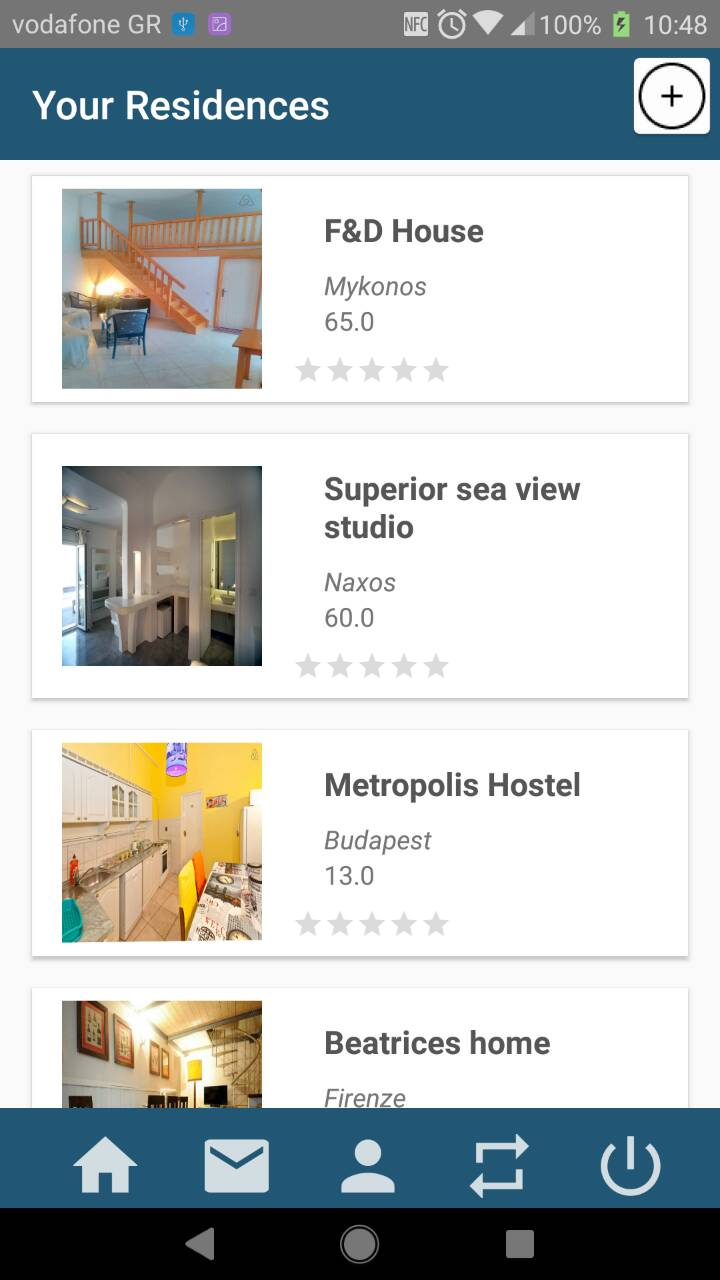
\includegraphics [scale = 0.18] {22-host.jpg}
			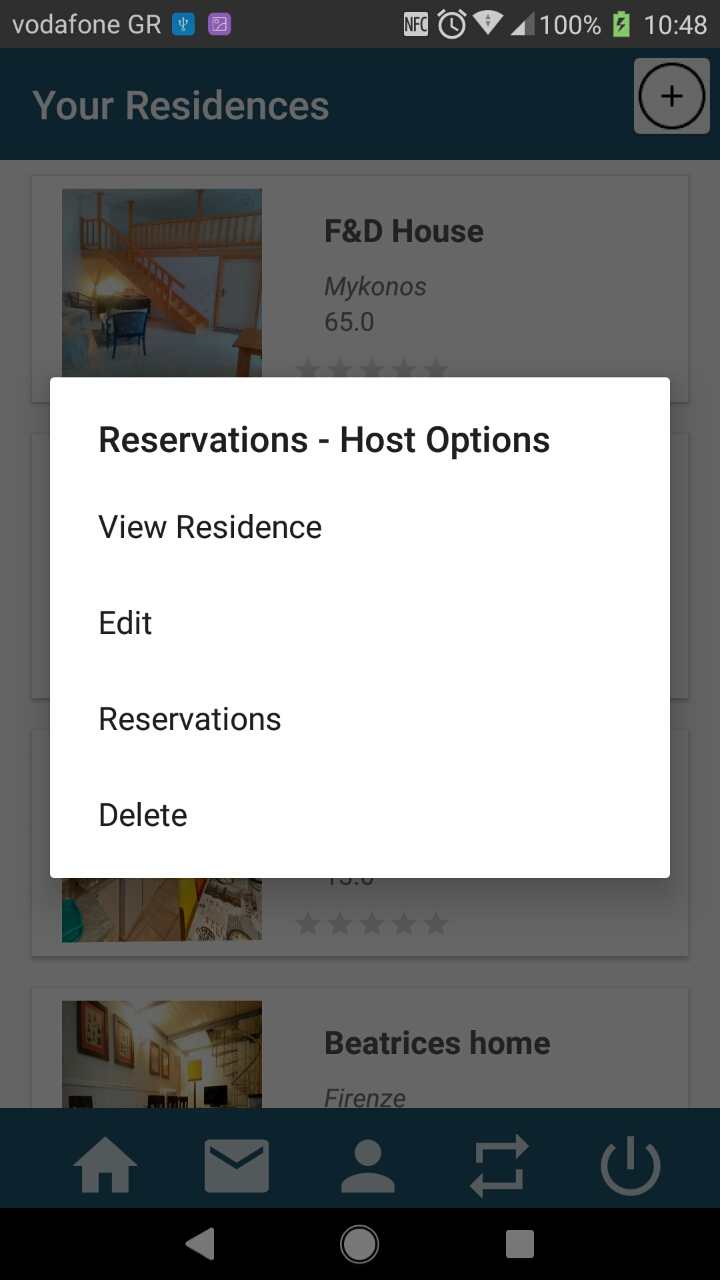
\includegraphics [scale = 0.18] {23-host.jpg}
			\caption{Host Activity}
		\end{center}
	\end{figure}
	
	\subsubsection{Add new Residence}
	On the top of the activity there is a toolbar with an add residence button. If this ImageButton is pressed, host is redirected to the \textit{AddResidenceActivity}, where he fills all requested fields with relevant information for the residence. It is mandatory to fill in all the fields, in order the upload to be accurate and present all the details to users. Here, user cannot upload any images, instead he can do it afterwards by editing his upload. When user completes all the fields, he is redirected to HostActivity, where now he can see his residence upload.
	
	\begin{figure} [H]
		\begin{center}
			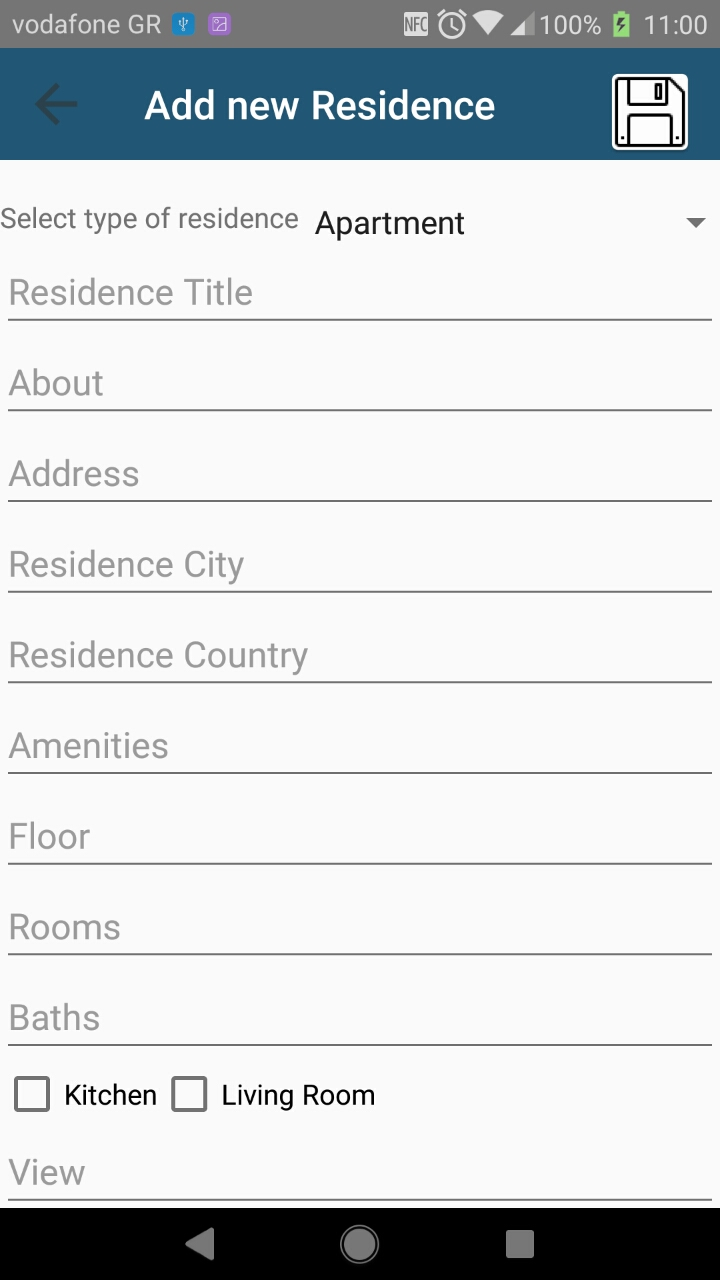
\includegraphics [scale = 0.18] {25-addResidence.jpg}
			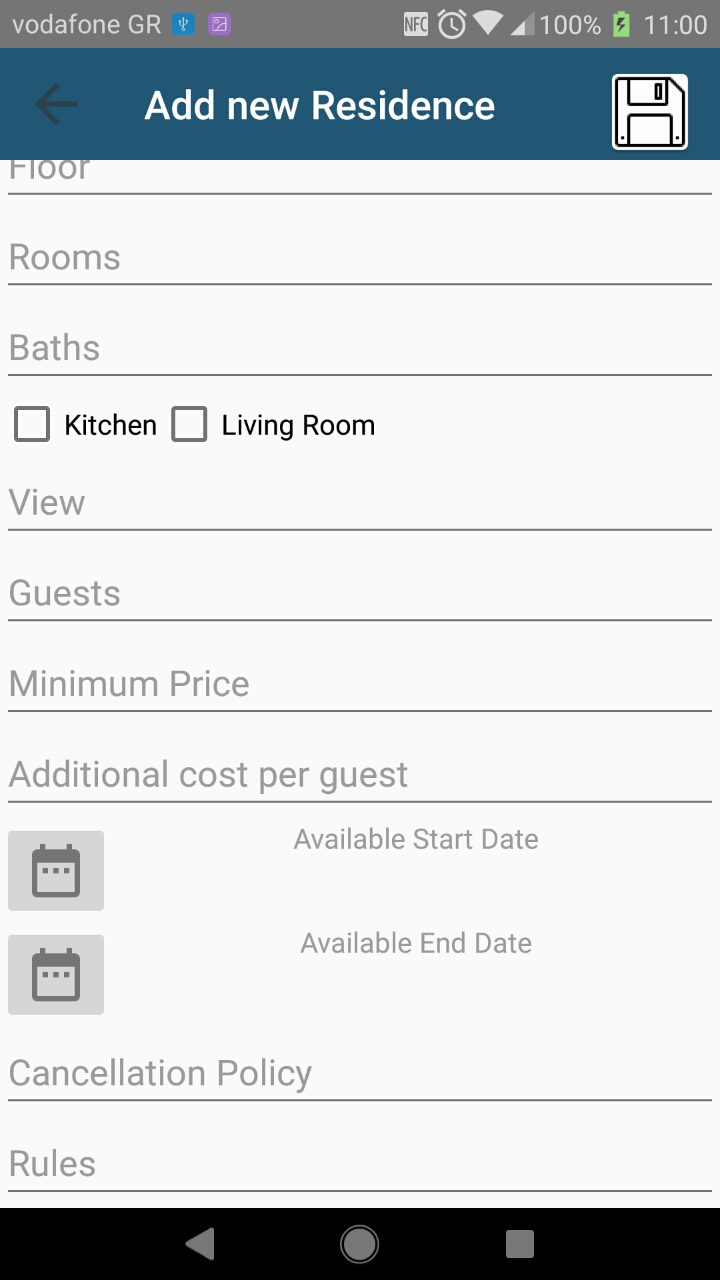
\includegraphics [scale = 0.18] {26-addResidence.jpg}
			\caption{Add Residence Activity}
		\end{center}
	\end{figure}
	
	\subsubsection{Edit Residence}
	If the host chooses to edit his residence, he is redirected to \textit{EditResidenceActivity}, with the same layout as the AddResidenceActivity, in the difference that now user can upload images.
	The procedure of uploading the image is the same as on the profile photo, only this time the user is able to select multiple images for the residence and not only one. This is happening with the help of an external library \textit{Android Multiple Images Selector} which formats a specific custom layout view to open a GridView of showing all the images stored in the device folders. In that way the user is able to select different images from different folders up to the limit that we have specified, which in this case is 5(images). After selection of the images, a Toast message appears notifying the user of the number of images pending to be uploaded. On clicking the save button the images start uploading into the server folder. The @MultiPart annotations are the same as on the profile image, only this time the image names are stored on the images\_table on the database. The id of the edited residence is taken and assigned to each row being saved on the table. The last image saved gives its' return custom name to the \textit{photos} field of the residence into the android. 
	
	The residence is being updated with the edited fields (@PUT request on RESTful Service) and the main residence photo that will be shown on the residence list is also declared. After a successful operation of the above the user is redirected to the main view of the host residences. Otherwise, if the token is expired, the logout method is called without saving the changes and user now goes to the GreetingActivity in order to login again.
	
	In case there are images already assigned to the residence, the user has the ability to edit them when entering the EditResidenceActivity through a context menu. Above the button \textit{Add Photos} we have set up an inner recycler view which lists all the relevant images and shows them in thumbnail size. Two options are available by long clicking each one. Delete it or set it as main image. By deleting the image, the \textit{images\_table} is updated, deleting the row with the specific name, and the image file is also deleted from the server side. By setting it as main, the \textit{photos} field from the current residence is updated with the name of the image being selected. In order to set some image as main, all the images must have been already stored in the images\_table and existing into the server folder.
	
	\begin{center}
		\begin{figure}
			\begin{tabular}{c c c}
				
				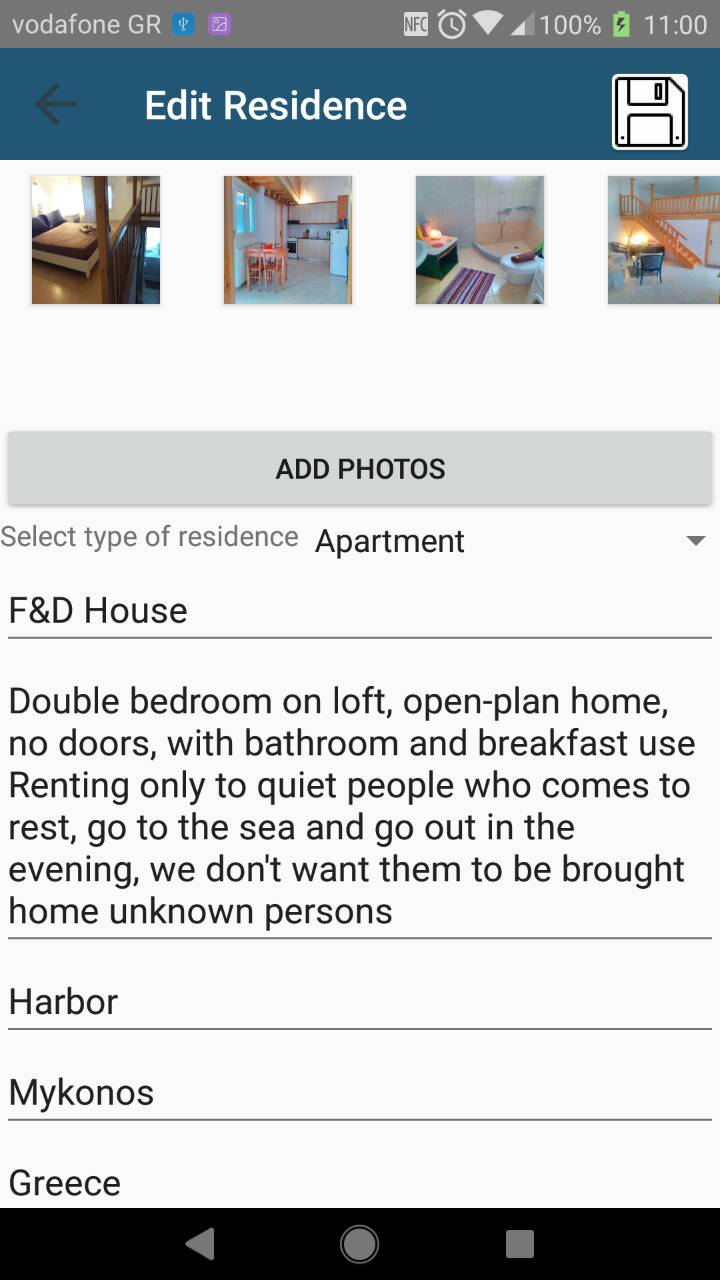
\includegraphics[scale=0.17, keepaspectratio]{27-editResidence.jpg}  
				&
				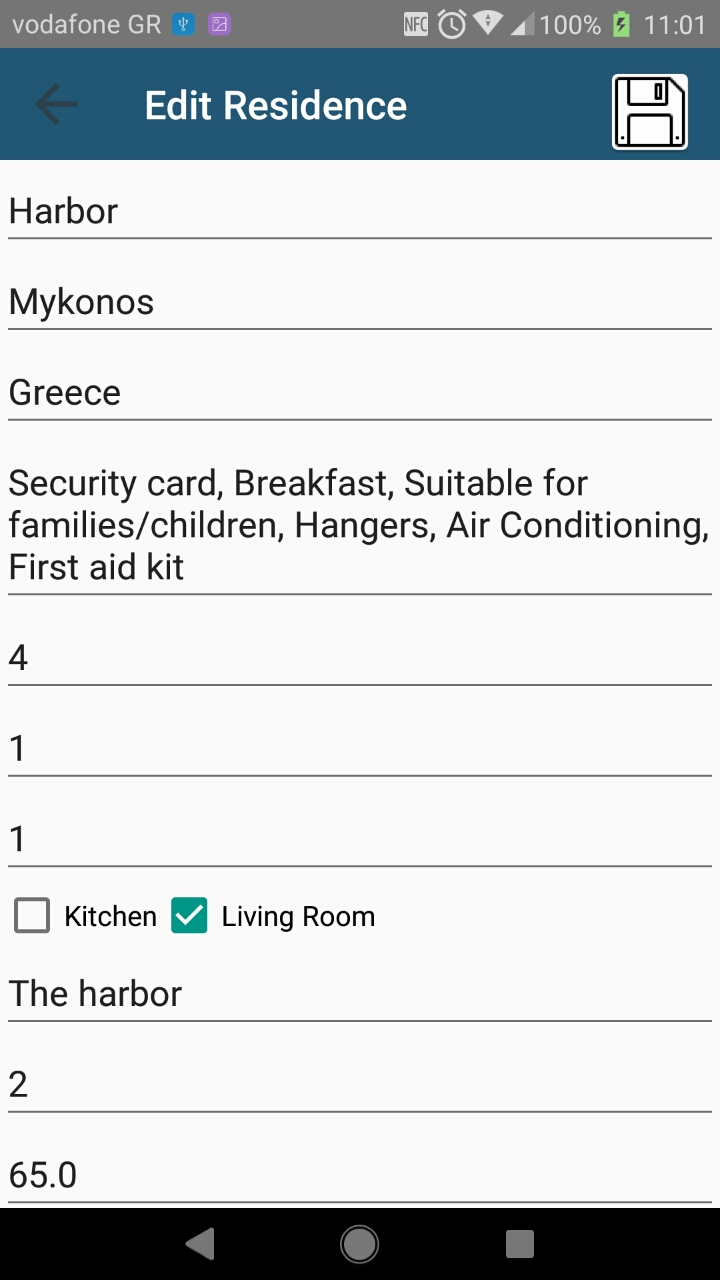
\includegraphics[scale=0.17, keepaspectratio]{28-editResidence.jpg}  
				&
				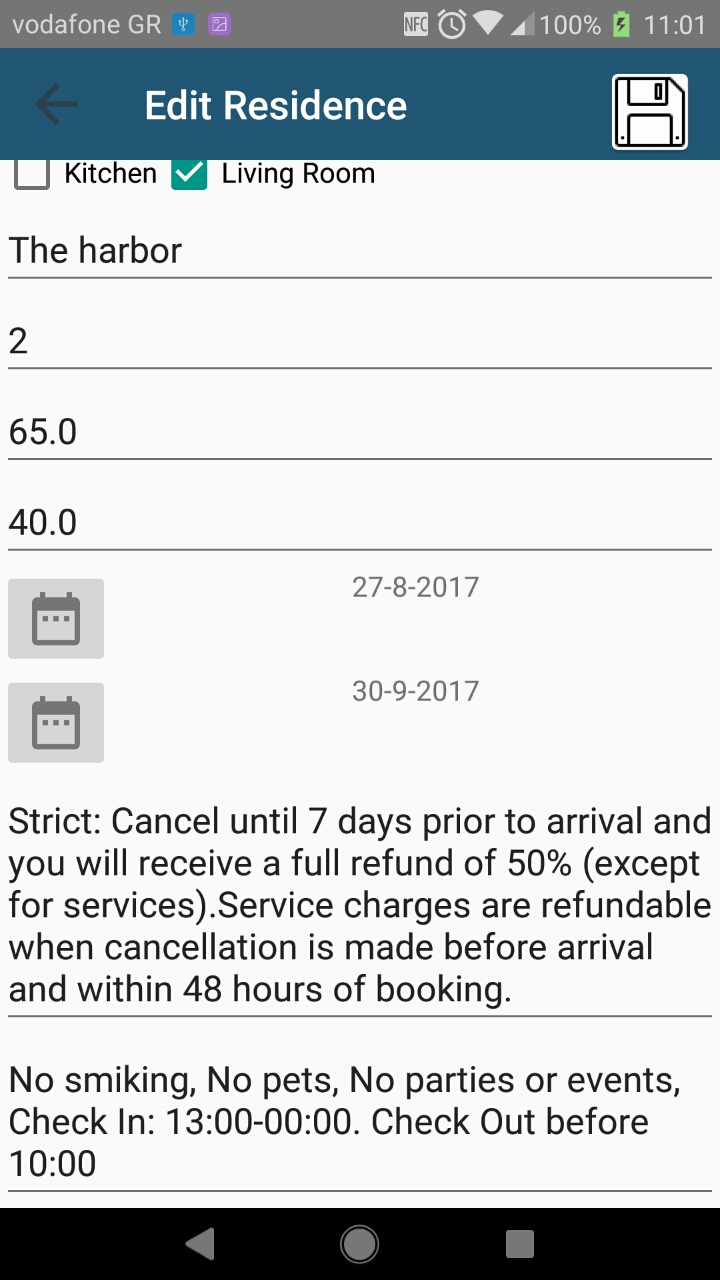
\includegraphics[scale=0.17, keepaspectratio]{29-editResidence.jpg}
				\\
			\end{tabular}
			\caption{Edit Residence Activity}
		\end{figure}
	\end{center}
	
	\subsubsection{Delete Residence}
	While host is in the HostActivity, he can choose a residence and from the context menu, he can press the delete option. This sends a DELETE request and the result is presented to user (who remains in the HostActivity) using a "Toast" and then this residence disappears from the list (using the recycler adapter and notifyDataSetChanged). Respectively, the reservations, reviews, and images tables are being updated, deleting all the values that are related to the specific residence.
	
	\section{Overview}
    Having completed the requirements of the project, we can conclude to a complete understanding of the implementation of an Android application. We have examined thoroughly the connection of an Android project and a RESTful API project with the use of web services. It is proven that an application is able to manage only the front functionalities that are visible to the user, and the background data management can happen from an external source (REST) without having a direct connection with the database. The communication between the RESTful Entities and the database constitutes a very critical point of a successful operation as every db change has to be exactly assigned to the REST side too. In order for the MySQL queries and every entity field to work correctly, we had to be very careful on the connection regarding the foreign keys, the insertion/rename/deletion of a table or a field and every other action that would affect the main data.
    
    We understood the basic logic around external libraries, helpful for the operation of either the application or the RESTful Service. From the side of android, the external libraries were able to be imported through a simple \textit{compile} command into the gradle file - of course by checking the versions and the validity of each one. From the side of the REST, there was a file import process into the Glassfish server - where it was also important any \textit{jar} file to be compatible with the configuration settings of the project. In both cases, we had to be careful on the declaration of these files, especially when we were sharing our project remotely.

    Moreover, during the examination of the project, from the very beginning, we noticed that small details might cause serious malfunction and therefore delay our progress. We came to knowledge that it is very important to guarantee the device status in combination with the properties of the whole project. First of all the network connection had to be the same in the android device but also in the REST API. This was an important criteria as our glassfish project was set up locally. In addition to that, there might be more restrictions occured, based on the operating system used (i.e. the Firewall). The version of the device shall also be compatible with the Sdk version that the android project supports. The main issue is to manage to run the application in different devices, no matter what the configuration steps will be.
    
    Through the Android application, we were able to expand more the project, by adding more functionalities that could facilitate and help the usage of the user, and that it is common to see in every other application these days. Below, we present some of the main issues we dealt with from both sides of the project, and that we had to adjust them and adopt a logic that would make the system operate, and on the same time would be valid and correct.

	\subsection{Date Format}
	Before the Retrofit 2.0 library was presented during the Android lessons, we have tried to perform the rest calls in the same way as we do for the map in ResidenceActivity. After the calls, a JSON object had been received and we mapped the fields with the fields of our objects (Users, Residences etc) manually. In this way we have not faced any problems with POST, PUT, GET etc calls, since we always checked the specific JSON result and then we mapped it to an objects field.
	
	However, after the inclusion of Retrofit to our project, all date fields in the database could not be filled correctly with POST and PUT requests. The way that Android was converting the input date in order to send it to the REST call, couldn't be recognized in any way. We have tried several solutions we found on the Internet (like using Gson converter in our RestClient) however, none of those solutions worked and we had null date values in all our tables. Therefore, we have decided to change the type of the date fields in the database. As a result, the RESTful Web Services project entities and the relevant android objects were built again. In Users table, we have declared the birth date as String since we use this date only for displaying it to the user, with no further action in the application side. Regarding all other dates used through the calendar, specifically Residences (available\_date\_start, available\_date\_end) and Reservations (start\_date, end\_date), we have decided to declare them as \textit{bigints}, from the side of database, which will be recognized as a \textit{long} type, from the side of the REST, and Android. As for the values \textit{timestamp} on Messages and \textit{registration\_date} on Users, there wasn't any need of changing them, as these fields are updated only on the database, changing their value to the current date and time at the moment.
	
	This bigint value that will be used, represents the data in a format type of a numeric timestamp of the date, converted in milliseconds. So practically, the saved data remains valid, only in different format. In this way, POST and PUT requests work properly and we can store dates in our database. Also, GET requests give us the expected results, but we have to transform all bigints and timestamps to dates on the Android side, in order to present them to user, since no better solution was found.
	
	\subsection{RecyclerView vs ListView}
	
	Following the instructions during the Android Lessons, we have used in almost all our activities a ListLayout, in order to display Residences, Reservations, Reviews etc to the user. However, while searching in the Internet, we found a more elegant and easy way to display lists, the RecyclerView.
	
	Therefore, we have decided to replace all our ListViews with a RecyclerView, except the one related to reviews. In this way, we provide only the ArrayList with our object to the adapter and not arrays with the fields of the object we want to display. Moreover, setters and getters can be used in order to update the ArrayList and notify the adapter instead of reloading the activity.
	
	Furthermore, apart from RecyclerView, CardView layout is used when presenting the results to user (except the MessageActivity), which improves a lot the layout in a more structured way. Related to the xml files, we have created a file with the recycler, which we include in all layout xml files that we want to use the recycler. Then, in java files we create one class with the adapter and the CardView and then in our activity we set the adapter and notify it when changes happen (e.g. delete a reservation).
	
	\subsection{Calendar - Caldroid}
	
	Although we have already mention the use of Caldroid in the Detailed Presentation of residences subsection, we believe that it is worth to be mentioned in this section with all the difficulties and technical decisions that have been made.
	
	With the use of the custom calender, we cannot select the start and end date for booking, therefore we have found on GitHub the Caldroid, which we use in a fragment (variable caldroidFragment in ResidenceActivity). This calendar lets us change the selected dates and also disable all fully booked, functionality that is not provided in the custom calendar of Android. Therefore, we use the information of dates from Residences and Reservations and the number of guests in Reservation and the one provided by the user in order to calculate the availability and decide if the user can be accommodated during the selected period. All this procedure can be found in setCalendar and filterDates methods. Finally, we use onSaveInstanceState, in case the app is minimized to keep the status of the calendar as it is.
	
	\subsection{Maps - SupportMapFragment - GoogleMap}
	
	In the same activity, we also present a map showing the location of the residence. In order to achieve this functionality, as already mentioned, we have requested a maps key from Google and then we have created the xml file \textit{google\_maps\_api} containing this key. In AndroidManifest, respective permission is created, using this key. In activity\_residence xml file, a fragment is used in order to contain the map.
	
	In our java code, we used the classes that we have created for Rest calls. Therefore, we use the sendGET method in order to send a request to the following link: \newline "https://maps.googleapis.com/maps/api/geocode/json", providing the address, city and Country of the residence as well as the Google Key, getting back a JSONObject. The rest we have described it in the subsection related to the detailed presentation of the residences. The method that sets the map is the onMapReady.
	
	\subsection{Token - Retrofit}
	
	One other important difficulty to be mentioned, is the way we consume the Restful services. When we first started to develop the application, we were not aware of the library Retrofit 2.0 and, as we have already mentioned, we have found another way to perform the calls. In more details, we have created a class named "RestCallParameters" that includes the request type (GET, POST, PUT, DELETE), the return type (JSON, XML, Plain Text) and, in case of POST requests, all the fields to be sent for posting in the database. Another class created is the RestCallManager, which includes the AsyncTask and checks the request type in order to call the proper method (sendGET, sendPOST etc) to perform the call. The method getSingleJSONArray gets the JSON Array from the GET call and stores in an ArrayList all the JSONObjects. In class RestCalls, we created a RestCallParamaters and a RestCallManager objects and also a relevant to the request method, that used to take the result from the getSingleJSONArray method and return respective object (Users, Residences etc). In the classes of those objects we have implemented a fromJSON and a toJSON methods in order to map the JSONObject to the fields of the relevant object.
	
	When the Retrofit library was presented, we have decided to replace the above logic with the Interface RestAPI, the class RestClient and the RetrofitCalls class with all the necessary calls for our application. This logic was far more easy and mapped automatically the object to the JSONObject.
	
	One other requirement of the project was to create a session to each register/login action. In the Restful services side, we create a token when the login and register methods are called and it is returned to the application. In all the other calls, the token is required as header and it is checked whether it is expired or not. The method returns the requested result if token is still valid, otherwise it returns "not".
	
	In the Android side, when the user performs a login or register call, the method getStringClient is called (from RestClient class) with empty header. These two calls return a new token to the application, which is stored in the SharedPreferences. In all other calls, the getClient method is called and the token is provided as parameter and used as header to this call.
	
	In addition, a method to check if token is expired, is implemented and called at the beginning of each activity. In all calls the token is sent in the header  so as to be checked in the Restful services side. When user chooses either to login or to register, a token is received from the Restful services and it is stored in a session object so as to be checked when an activity starts. In the class RetrofitCalls, in all methods implemented, we provide the token to be also checked in the Restful services side. Finally, if Android finds out that the token is expired, the logout method is called, user is redirected to the GreetingActivity and a Toast message appears to inform him that the session has expired.
	
	\subsection{Confidential REST calls - SSL}
	Based on the requirements of the project, there was a need to be able to make safe calls between the Android and the RESTful services. A main logic into RestClient (getUnsafeOkHttpClient method) was implemented, managing to send and accept calls from urls supported with SSL. On the other hand, the REST should also be able to make itself valid, and pass its calls only through HTTPS. This was managed through the configuration of security-constraint properties into the web.xml file of the REST api project.
	
	The web.xml file contains information about the structure and external dependencies of web components in the module and describes how the components are used at run time. To enable the web container to run Java API for RESTful Web Services applications, we configured the web.xml file to point directly to the current servlet. In order to make it SSL valuable, we filled the generated xml with an Encryption tag, setting it as confidential between user data constraints. As a result, the api is deployed and runs only under SSL authorization, having moved its port from 8080 to 8181.
	
	\begin{itemize}
		\item\textbf{Single Image View:} This change caused the images to not be able to load correctly on the Android side. This was happening because the image url (REST call) from the library Picasso was called directly and not through RestClient in order to verify the SSL encryption. Therefore, as a solution, we have implemented the PicassoTrustAll class, which uses the OkHttp library and in this way the application can get all images from the server. So the single image loading managed to work correctly, but not on images slider too, as the library being used there is also different dealing also with a direct url call.
		
		\item\textbf{Images Slider View:} In order to show all images of a residence in the ResidenceActivity, we have used a \href{https://github.com/daimajia/AndroidImageSlider}{slider found in GitHub}. However, as mentioned above, we faced the same problem with image loading due to SSL encryption. The solution we came up with in order to solve this issue, was to override two classes of this library: the TextSliderView and the BaseSliderView. Therefore, we have created the MyBaseSliderView and the MyTextSlider class which extends the first one. Our goal was to replace the Picasso object, created for each image, with the PicassoTrustAll in order to include the OkHttp client. For this purpose, we have overridden the method bindEventAndShow in our MyBaseSliderView class, the value of myPicasso object is set to an instance of PicassoTrustAll.
	\end{itemize}
	
	\subsection{Messages - Notifications}
	Having implemented a logic of a chat conversation between the users, giving them the ability to check which of their conversations are unread or not, we have set up a notification logic through the benefits of Android, in order for the application to notify the user when they have a new message, no matter if they use the app or have it minimized. More specifically, we implemented a private class "Worker" into the HomeActivity, which is called only when it is verified that the user is logged in. This Worker class works in the background of the application using the overridden methods doInBackground and onPostExecute. It makes a call on an initialized TimerTask which makes a @GET call on the RESTful service every four minutes checking for the number of unread messages into every active conversation of the current logged in user. if the number of unread conversations is higher than zero, a notification bar appears on top of the screen as shown below.
    
    Nevertheless, there was a conflict during the background check of the notifications. Having in mind that the Worker class was implemented into the Home activity, in order to get every important data required for the user, the TimerTask was called every time the HomeActivity was called. In order to avoid this, we implemented a Shared Preference to a boolean value \textit{workerRuns} which is set to false by default - so the first time the home screen loads, the Worker will start too. Once the Worker starts, workerRuns is set to true - so the next time the onResume method (HomeActivity.java) is called, it will ignore the initialization of the Worker. We also manage to clear the Shared Preference in cases when the user logs out of the application, or their token gets expired. In that way, they avoid getting notifications of not valid data.
	
	\begin{figure} [H]
		\begin{center}
			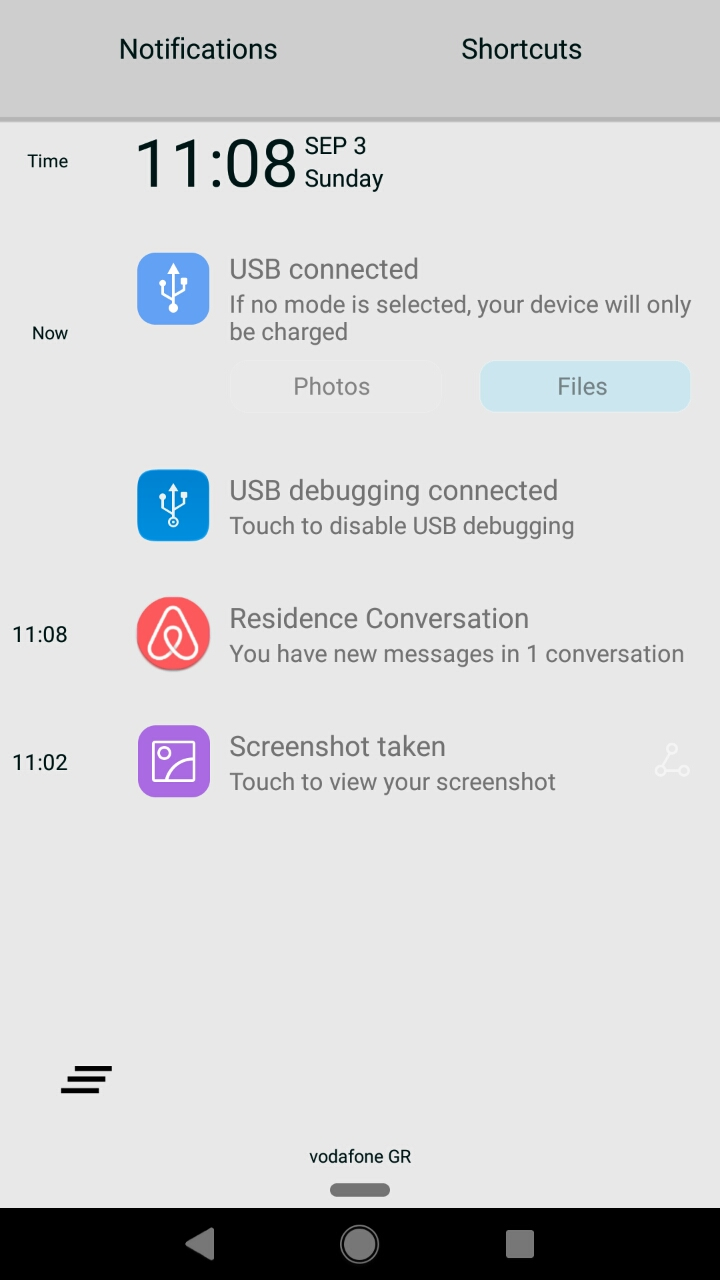
\includegraphics [scale = 0.18] {notification.jpg}\\[1.0 cm]
			\caption{Screenshot of notification}
		\end{center}
	\end{figure}
	
	The user can dismiss this notification or click on it and get navigated directly into the InboxActivity screen, where they can see how many conversations they haven't opened yet. It is important to mention that this functionality works correctly only when the application is already working. No matter if the user minimizes the app or has it resumed on some screen, even different from Home, the background timer works and pops up the notification when needed. Of course, when the user opens a conversation (and the read value is changed to one), the next time the handler of the timer executes, it will count one less unread conversation and therefore, change its' value.
	
	\subsection{REST calls - Cached values}
	Another important issue that occurred during the implementation of the project, was the returned result after @POST or @PUT requests. This issues was observed on the images uploading functionality, where together with the saving on the server folder, we were making one more call to the database, updating either the images\_table (with residence images) or the users\_table (with profile images). Even though the database was correctly informed and updated after one such request, and the files have been saved successfully to the folder, the data being returned after a @GET method wasn't correctly informed. For example, after a successful edit and a new profile photo selected on the user profile (EditProfileActivity), when the user is redirected to the ProfileActivity they have to see all the fields informed with the latest update. Instead, the image is not correct - it might have the previous still shown (even if it was deleted from the server and got replaced from the new one) or have no image at all (if the user uploaded an image for the first time) - even if all the rest fields are correctly updated. This was a hint of a cache problem that had nothing to do with android, as making a direct call to the RESTful method (from a web browser for example) was still returning a cached value.
	
	This problem was happening only on the section of images, because only there, there was an interaction with the local files of the server (the images folder) which are being cached and update their content every few minutes. When the user edits their profile or residence, they can't see immediately their changed photos, although when they check their application after a few minutes, and reload their screen again, they will see them updated. This is a very normal case of a cache implementation logic in order to avoid latency of bringing the data or having to interact with the Glassfish server continuously. 
	
	However, in our case the things are different, as we are dealing with a mobile application, not a web, and therefore the management of that is more strict. After having searched thoroughly, adding Cache-Control Headers into our requests and setting up checks of the existence of the last modified date inside the method, or the expiration of the date in order to load new data, we haven't managed resolving the issue. After all, the solution was hidden in a separate setting which was restricting the api from recognizing the changes. As this RESTful project is implemented, several files have been configured in order to set up its' whole structure, the connection with the database (\textit{glassfish-resources.xml}), the SSL encryption of the REST URI (\textit{web.xml}) and lastly, the management of the whole api settings in combination with the involvement of the jersey library where the files uploading functionality is based on (\textit{persistence.xml}). So as it seemed, the main issue, was to specify the \textit{Shared Cached Mode} Unit to None in order to avoid caching the files and instead show the cleared result immediately.
	
	Such technique isn't recommended in general, as caching values and data is a perfect way of not "burdening" the application with constant calls to the database. But for the purpose of our project, the main need is to check and show the correct data at the time needed.
	
	\newpage
	\addcontentsline{toc}{section}{References}
	\begin{thebibliography}{30}
		\bibitem{knuthwebsite} \href{https://netbeans.org/kb/docs/websvc/rest.html}{Getting Started with RESTful Web Services}
		\bibitem{knuthwebsite} \href{http://www.naun.org/main/NAUN/computers/16-579.pdf}{XML-RPC vs SOAP vs REST web services in Java, uniform using WSWrapper}
		\bibitem{knuthwebsite} \href{https://futurestud.io/tutorials/retrofit-synchronous-and-asynchronous-requests}{Retrofit — Synchronous and Asynchronous Requests}
		\bibitem{knuthwebsite} \href{https://inthecheesefactory.com/blog/retrofit-2.0/en}{Retrofit 2.0}    
		\bibitem{knuthwebsite} \href{https://spring.io/guides/gs/consuming-rest-android/}{Consuming a RESTful Web Service with Spring for Android}
		\bibitem{knuthwebsite} \href{https://developer.android.com/reference/android/os/AsyncTask.html}{AsyncTask}
		\bibitem{knuthwebsite} \href{https://developer.android.com/topic/libraries/architecture/guide.html}{Guide to App Architecture}    
		\bibitem{knuthwebsite} \href{https://developer.android.com/training/appbar/actions.html}{Adding and Handling Actions}    
		\bibitem{knuthwebsite} \href{http://www.androidinterview.com/android-custom-listview-with-image-and-text-using-arrayadapter/}{Android Custom Listview with Image and Text using ArrayAdapter}    
		\bibitem{knuthwebsite} \href{https://www.androidhive.info/2016/01/android-working-with-recycler-view/}{Android Working with Recycler View}
		\bibitem{knuthwebsite} \href{https://github.com/roomorama/Caldroid}{Caldroid}    
		\bibitem{knuthwebsite}  \href{https://stackoverflow.com/questions/40185331/how-to-use-context-menu-on-recyclerview-item-provided-by-firebaseui}{ContextMenu in RecyclerView}
		\bibitem{knuthwebsite} \href{http://square.github.io/picasso/}{Picasso}
		\bibitem{knuthwebsite} \href{https://github.com/daimajia/AndroidImageSlider}{Android Image Slider}
		\bibitem{knuthwebsite} \href{https://github.com/zfdang/android-multiple-images-selector}{Android Multiple Images Selector}
		\bibitem{knuthwebsite} \href{https://developer.android.com/training/maps/index.html}{Adding Maps}
		\bibitem{knuthwebsite} \href{https://developers.google.com/maps/documentation/android-api/map-with-marker}{Adding a Map with Marker}
		\bibitem{knuthwebsite} \href{https://developers.google.com/maps/documentation/android-api/current-place-tutorial}{Select Current Place and Show Details on a Map}
		\bibitem{knuthwebsite} \href{https://developer.android.com/guide/topics/ui/notifiers/notifications.html}{Notifications}
		\bibitem{knuthwebsite} \href{https://developer.android.com/training/notify-user/build-notification.html}{Building a Notification}
		\bibitem{knuthwebsite} \href{https://www.tutorialspoint.com/restful/restful\_caching.htm}{RESTful Web Services - Caching}
		\bibitem{knuthwebsite} \href{https://devcenter.heroku.com/articles/jax-rs-http-caching}{HTTP Caching in JAVA}
		\bibitem{knuthwebsite} \href{http://www.oracle.com/technetwork/articles/java/persistenceapi-135534.html}{Using the Java Persistence API in Desktop Applications}
		
		
	\end{thebibliography}
	
\end{document}